% $Id$

In this chapter we review some of the physics underlying the detection of
gravitational waves from binary inspiral.  In section~\ref{s:effect} we review
the effect of gravitational waves on a pair of freely falling particles in
order to introduce some of the concepts that we need to discuss the detection
of gravitational waves from binary inspiral.  For a detailed description of
gravitational waves, we refer to \cite{MTW73,Thorne:1982cv}.
Section~\ref{s:ifos} describes how a laser interferometer can be used to
measure this effect. The gravitational waveform produced by the inspiral of
two compact objects, such as neutron stars or black holes, are discussed in
section \ref{s:inspiralgw}. We also derive the waveform that will be used to
search for gravitational waves from binary inspiral events in the Universe.

\section{The Effect of Gravitational Waves on Freely Falling Particles}
\label{s:effect}

The 4-velocity $\vec{u}$ of a freely falling test particle satisfies the
geodesic equation\cite{Wald:1984}
\begin{equation}
\label{eq:geodessic}
\left(\nabla_{\vec{u}} \vec{u}\right)^\alpha =
\tensor{u}{^\alpha_{;\mu}}u^{\mu} = 0,
\end{equation}
where $;$ denotes the covariant derivative, that is,
\begin{equation}
\tensor{u}{^\alpha_{;\mu}}\tensor{u}{^{\mu}} = \left(\tensor{u}{^\alpha_{,\mu}} +
\Gamma^\alpha_{\mu\nu}u^\nu\right) u^\mu,
\end{equation}
where $\Gamma^\alpha_{\mu\nu}$ is the connection coefficient of the metric
$g_{\mu\nu}$ and $,\mu$ represents the standard partial derivative with
respect to the coordinate $x^\mu$. 

Consider two particles $A$ and $B$, as shown in figure \ref{f:particles}~(a),
with separation vector $\vec{\xi}$. The particles are initially at rest with
respect to each other, so
\begin{align}
\nabla_{\vec{u}} \vec{u} &= 0, \\
\vec{u} \cdot \vec{\xi} & = 0.
\end{align}
If the spacetime is curved, the second derivative of $\vec{\xi}$ along
$\vec{u}$ is non-zero; it is given by the equation of geodesic deviation
\begin{equation}
\nabla_{\vec{u}}\nabla_{\vec{u}} \vec{\xi} = -
R(\_,\vec{u},\vec{\xi},\vec{u}),
\end{equation}
where $R(\_,\vec{u},\vec{\xi},\vec{u})$ is the Riemann curvature tensor. 
If the spacetime is flat with weak gravitational waves propagating in it, we
can describe it by a metric 
\begin{equation}
g_{\mu\nu} = \eta_{\mu\nu} + h_{\mu\nu},
\end{equation}
where $h_{\mu\nu}$ is the perturbation to the metric due to the gravitational
waves and $\eta_{\mu\nu}$ is the flat Minkowski metric .  We now introduce a
\emph{Local Lorentz Frame} (LLF) for particle $A$.  The LLF of particle $A$ is
a coordinate system $x^\alpha$ in which
\begin{equation}
g_{\mu\nu}(A) = \eta_{\mu\nu}
\end{equation}
and
\begin{equation}
g_{\mu\nu,\alpha}(A) = 0,
\end{equation}
where $g_{\mu\nu}(A)$ is the value of the metric at point $A$. This LLF
is equivalent to a Cartesian coordinate system defined by three orthogonally
pointing gyroscopes carried by particle $A$. The curvature of spacetime means
that the coordinate system is not exactly Cartesian, but it can be shown that
this deviation is second order in the spatial distance from the
particle\cite{MTW73}. This means that along the worldline of particle $A$ the
metric is
\begin{equation}
g_{\mu\nu} = \eta_{\mu\nu} + \frac{\mathcal{O}\left(|\vec{x}|^2\right)}{R^2}
\end{equation}
where $\vec{x}$ is the distance from the particle and $R \sim
|R_{\alpha\beta\gamma\delta}|$. We can write the Cartesian coordinates of the
LLF of $A$ as $x^\mu = (x^0,x^i)$, where $x^0 = t$ is the timelike coordinate
and $x^i$ are the three Cartesian coordinates. Then in
the LLF of particle $A$ the equation of geodesic deviation becomes
\begin{equation}
\frac{\partial^2 \xi^{j}}{\partial t^2} = -
\tensor{R}{^j_{\alpha\beta\gamma}}u^\alpha\xi^\beta u^\gamma =
-\tensor{R}{^j_{0k0}} \xi^k,
\end{equation}
since $u = (1,0,0,0)$.  The presence of the gravitational waves are encoded in
the curvature $R_{\alpha\beta\gamma\delta}$ which satisfies the wave equation
\begin{equation}
\eta^{\mu\nu}R_{\alpha\beta\gamma\delta,\mu\nu} = 0.
\end{equation}
In the Local Lorentz frame, the components of $\vec{\xi}$ are just the
coordinates of $B$.  
In the LLF of $A$ we may write
\begin{equation}
\label{eq:bcoords}
\xi^j = \xi_{(0)}^j + \delta \xi^j,
\end{equation}
where $\xi_{(0)}^j$ is the unperturbed location of particle $B$ and $\delta
\xi^j$ is the change in the position of $B$ caused by the gravitational wave.
Substituting equation (\ref{eq:bcoords}) into the equation of geodesic
deviation, we obtain
\begin{equation}
\label{eq:particledev}
\frac{\partial^2 \delta \xi^j}{\partial t^2} \approx - \tensor{R}{^j_{0k0}} \xi_{(0)}^k =
-R_{j0k0} \xi_{(0)}^k,
\end{equation}
where we have used $\eta_{\mu\nu}$ to lower the spatial index $j$ of the
Riemann tensor. For a weak gravitational wave, all the components of
$R_{\alpha\beta\gamma\delta}$ are completely determined by $R_{j0k0}$.
Furthermore, it can be shown that the $3\times3$ symmetric matrix $R_{j0k0}$,
which we would expect to have $6$ independent components, has only $2$
independent components due to the Einstein equations and the Biancci identity.
We define the (transverse traceless) gravitational wave field,
$h_{jk}^\mathrm{TT}$, by
\begin{equation}
-\frac{1}{2} \frac{\partial^2 h_{jk}^\mathrm{TT}}{\partial t^2} \equiv
R_{j0k0}^\mathrm{TT}.
\label{eq:hjkdef}
\end{equation}
Using this definition in equation (\ref{eq:particledev}), we obtain
\begin{equation}
\delta \xi^j = \frac{1}{2} h_{jk}^\mathrm{TT} \xi_{(0)}^k.
\label{eq:gwxeffect}
\end{equation}
If we orient our coordinates so the gravitational waves propagate in the
$z$-direction, so $h_{jk}^\mathrm{TT}(t-z)$, then the only non-zero components
of $h_{jk}^\mathrm{TT}$ are $h_{xx}^\mathrm{TT}$, $h_{yy}^\mathrm{TT}$,
$h_{xy}^\mathrm{TT}$ and $h_{yx}^\mathrm{TT}$. Since $h_{jk}^\mathrm{TT}$ is
symmetric and traceless, these components satisfy
\begin{align}
h_{xx}^\mathrm{TT} &= - h_{yy}^\mathrm{TT}, \\
h_{xy}^\mathrm{TT} &= h_{yx}^\mathrm{TT}.
\end{align}
For two more particles $C$ and $D$ separated by
\begin{equation}
\zeta^j = \zeta^j_{(0)} + \delta \zeta^j,
\end{equation}
as shown in figure \ref{f:particles} (b), the effect of the gravitational wave
is then given by 
\begin{equation}
\delta \zeta^j = \frac{1}{2} h_{jk}^\mathrm{TT} \zeta_{(0)}^k.
\label{eq:gwyeffect}
\end{equation}
Taking the two particles $A$ and $B$ to lie on the $x$-axis of the LLF of
particle $A$ with separation $x_{(0)}$, without loss of generality, we may
write
\begin{equation}
\xi = (x_{(0)} + \delta x,0,0),
\label{eq:gwxcoord}
\end{equation}
where $\delta x$ is the displacement of particle $B$ caused by the
gravitational wave. Similarly, if particles $C$ and $D$ lie on the $y$-axis of
the LLF of particle $C$ with separation $y_{(0)}$, we may write
\begin{equation}
\zeta = (0,y_{(0)} + \delta y,0)
\label{eq:gwycoord}
\end{equation}
where $\delta y$ is the displacement of particle $D$ caused by the
gravitational wave. 

We define the two independent components of the gravitational wave to be
\begin{align}
h_{+} &= h_{xx}^\mathrm{TT} = - h_{yy}^\mathrm{TT}, \\
h_{\times} &= h_{xy}^\mathrm{TT} = h_{yx}^\mathrm{TT}
\end{align}
which we call the \emph{plus} and \emph{cross} polarizations of the
gravitational wave respectively.  The influence of a linearly $+$ polarized
gravitational wave propagating in the $z$-direction on the particles $A,B,C,D$
is then given by substituting equations (\ref{eq:gwxcoord}) and
(\ref{eq:gwycoord}) into (\ref{eq:gwxeffect}) and (\ref{eq:gwyeffect})
respectively to obtain
\begin{align}
\delta x(t-z) &= \frac{1}{2} h_{xx}^\mathrm{TT}(t-z) x_{(0)},\\
\delta y(t-z) &= -\frac{1}{2} h_{yy}^\mathrm{TT}(t-z) y_{(0)}
\end{align}
Similarly, for a linearly $\times$ polarized gravitational wave propagating in the
$z$-direction the effect on the particles is
\begin{align}
\delta x(t-z) &= \frac{1}{2} h_{xy}^\mathrm{TT}(t-z) y_{(0)},\\
\delta y(t-z) &= \frac{1}{2} h_{yx}^\mathrm{TT}(t-z) x_{(0)}.
\end{align}
Figure \ref{f:rings} shows the effect of $h_{+}$ and $h_{\times}$ on a ring
of particles that lie in the $xy$ plane. We can see for the plus polarization
that the effect of a gravitational wave is to stretch the ring
in the $x$ direction, while squeezing it in the $y$ direction for the first
half of a cycle and then squeeze in the $x$ direction and stretch in the $y$
direction for latter half of the cycle.  There is therefore a relative change
in length between the two particles $AB$ and $CD$ as a gravitational wave
passes.  The overall effect of a gravitational wave containing both polarizations
propagating in the $z$ direction is
\begin{align}
\label{eq:deltax}
\delta x(t-z) &= \frac{1}{2}\left[h_{+}(t-z) x_{(0)} + h_{\times}(t-z) y_{(0)}\right],\\
\delta y(t-z) &= \frac{1}{2}\left[-h_{+}(t-z) y_{(0)} + h_{\times}(t-z) x_{(0)}\right].
\label{eq:deltay}
\end{align}
It is the change in the distance between a pair of particles that we attempt
to measure with gravitational wave detectors. We can see from equation
(\ref{eq:deltay}) that the change in length is proportional to the original
distance between the test masses. For a pair of test masses separated by a
length $L$, we define the \emph{gravitational wave strain} $h$ to be the
fractional change in length between the masses
\begin{equation}
h \equiv \frac{1}{2} \frac{\Delta L}{L}.
\end{equation}
The reason to include a factor of $1/2$ in this definition will become
apparent when we discuss measuring gravitational wave strain with an
interferometer.  
%If $x_{(0)} = y_{(0)} = L$ then the total strain produced by the gravitational
%wave described in equations (\ref{eq:deltax}) and (\ref{eq:deltay}) is defined
%to be the difference in the 
%\begin{equation}
%h = \frac{ \delta x - \delta y}{L}.
%\end{equation}


\section{The LIGO Gravitational Wave Detectors}
\label{s:ifos}

Several major efforts are
underway\cite{Barish:1999,Acernese:2002,Luck:1997hv} to measure the strain
produced by a gravitational wave using \emph{laser interferometry}. The
results in this thesis are based on data from the Laser Interferometer
Gravitational wave Observatory (LIGO). LIGO operates three
\emph{power-recycled-Fabry-Perot-Michelson} interferometers in the United
States. Two of these are co-located at the LIGO Hanford Observatory, WA (LHO)
and one at the LIGO Livingston Observatory (LLO). The interferometers at LHO
are 4~km and 2~km in arm length and are referred to as H1 and H2,
respectively. The interferometer at LLO is a 4~km long interferometer referred
to as L1. The locations and names of the detectors are shown in figure
\ref{f:usmap}.  As we saw in chapter \ref{ch:introduction}, to detect the
gravitational wave strain produced by typical astrophysical sources we need to
measure $h \sim 10^{-22}$. If we separate our test masses by a distance of
$4$~km (a practical distance for earthbound observatories) the challenge
faced by gravitational wave astronomers is to measure changes of length of
order
\begin{equation}
\Delta L \sim 10^{-22} \times 10^4\,\mathrm{m} \sim 10^{-18}\,\mathrm{m}.
\end{equation}

\subsection{The Design of the LIGO Interferometers}
\label{ss:ligoifos}

In an interferometric gravitational wave detector the freely falling masses
described in the previous section are the mirrors that form the arms of the
interferometer\footnote{The mirrors in an Earth bound gravitational wave
observatory are not truly freely falling as they are accelerated by the
gravitational field of the Earth. It can be shown that the horizontal motion
of suspended mirrors is the same as that of freely falling test masses.} and
laser light is used to measure the change in length between the mirrors.  The
challenge facing experimenters constructing a gravitational wave
interferometer is to measure changes of length of order $\sim
10^{-18}\,\mathrm{m}$ using laser light has a wavelength of $\lambda_l \sim
10^{-6}$~m.  It should be noted that measuring a phase shift
\begin{equation}
\Delta \Phi \sim \frac{\Delta L}{\lambda_l} \sim 10^{-12}
\end{equation}
is a factor $10^{12}$ more sensitive than the interferometers used by
Michelson and Morely to disprove the existence of the ether.

A schematic of a \emph{simple Michelson} interferometer is illustrated in
figure~\ref{f:ifodesign}~(a).  Laser light is shone on a \emph{beam
splitter} which reflects half the light into the \emph{$x$-arm} and transmits
half the light into the \emph{$y$-arm} of the interferometer. The light
travels a distance $L$ in each arm and then is reflected back towards the beam
splitter by the \emph{end test masses}. These masses are equivalent to the
test masses $B$ and $D$ in section~\ref{s:effect}.  Consider the light in the
$x$-arm. For the laser light, the spacetime interval between the beam splitter
and the end test mass is given by
\begin{equation}
ds^2 = g_{\mu\nu}\, dx^\mu\, dx^\nu = 0.
\label{eq:dist}
\end{equation}
In the presence of a plus polarized, sinusoidal, gravitational wave traveling
in the $z$-direction, equation (\ref{eq:dist}) becomes
\begin{equation}
c^2 dt^2 = \left[1 + h_{+}(t-z)\right] dx^2 + \left[1 - h_{+}(t-z)\right] dy^2 + dz^2.
\end{equation}
We can measure the response of the interferometer to a gravitational wave by
considering the phase shift of light in the arms. The phase that the light
acquires propagating from the beam splitter to the $x$-end test mass and
back is given by\cite{Saulson:1994}
\begin{equation}
\begin{split}
\Phi_x &= \int_0^{\tau_\mathrm{RT}} 2\pi f_l\, dt \\
&= \frac{1}{c} \int_0^L 2\pi f_l \sqrt{1 + h_{+}}\,dx -
\frac{1}{c} \int_L^0 2\pi f_l \sqrt{1 + h_{+}}\,dx \\
&\approx \frac{4\pi f_l L}{c} \left(1 + \frac{h_{+}}{2}\right),
\end{split}
\end{equation}
where $\tau_\mathrm{RT}$ is the round trip time of the light and $f_l$ is
its frequency. We have discarded higher order terms in $h_+$ as their effect
is negligible.  We can see that the phase shift acquired in the $x$-arm due to the
gravitational wave is
\begin{equation}
\delta \Phi_x = \frac{2\pi}{\lambda_l} h_{+} L.
\end{equation}
A similar calculation shows that the phase shift acquired in the $y$-arm is
\begin{equation}
\delta \Phi_y = - \frac{2\pi}{\lambda_l} h_{+} L
\end{equation}
and so the difference in phase shift between the arms is
\begin{equation}
\Delta \Phi = \frac{4\pi}{\lambda_l} h_{+} L.
\end{equation}
A typical astrophysical source of gravitational radiation of interest to LIGO,
has a frequency $f_\mathrm{GW} \sim 100$~Hz. Therefore the wavelength of the
gravitational wave is $\lambda_\mathrm{GW} \sim 3000$~km. If
$\tau_\mathrm{RT} = 1 / f_\mathrm{GW}$ there will be no phase shift of the
light at leading order in $h_+$. The light spends exactly one gravitational
wave period in the arm and so the phase shift acquired by positive values of
$h_+(t-z)$ is canceled out by the phase shift due to negative values of
$h_+(t-z)$. The interferometer achieves maximum sensitivity when the light
spends half a gravitational wave period in the arms, that is
\begin{equation}
L = \frac{\lambda_\mathrm{GW}}{2} \sim 1000\,\mathrm{km}
\end{equation}
which is a hopelessly impractical length for a earthbound detector. Instead,
a simple Michelson interferometer is enhanced by placing two additional
mirrors in the arms of the interferometer near the beam splitter, as shown in
figure~\ref{f:ifodesign}~(b). These inner $x$ and $y$ test masses (referred to
as ITMX and ITMY) are designed in LIGO to store the light in the arms for
approximately one half of a gravitational wave period.  The mirrors create a
\emph{Fabry-Perot cavity} in each arm that stores the light for $B \sim 200$
bounces, giving a phase shift of
\begin{equation}
\Delta \Phi = 4\pi \frac{L}{\lambda_l} B h_{+} \sim 
10 \times \frac{4 \times 10^3\,\mathrm{m}}{10^{-6}\,\mathrm{m}} 
\times 200 \times h_+.
\end{equation}
For a gravitational wave strain of $h \sim 10^{-22}$, this increases
$\Delta\Phi$ by 3 orders of magnitude to a phase shift $\Delta \Phi \sim
10^{-9}$.  Further increasing $B$ does not gain additional sensitivity,
however, as storing the light for longer than half a gravitational wave period
causes it to lose phase shift as the sign of the gravitational wave strain
changes.

Is it possible to measure a phase shift of $10^{-9}$ using a
Fabry-Perot-Michelson interferometer? We measure the phase shift by averaging
the light at the photodiode over some period, $\tau$. Let $N$ be the number of
photons from the laser arriving at the photodiode in the time $\tau$. The
measured number of photons in the averaging interval is a Poisson process,
with probability distribution function for $N$ given by
\begin{equation}
p(N) = \frac{ \bar{N} ^{N} \exp \left(-\bar{N}\right) } {N!},
\end{equation}
where $\bar{N}$ is the mean number of photons per interval $\tau$.
%A very
%large number of photons, $N_\gamma \gg 1$, will arrive at the photodetector in
%the averaging time, however, so this Poisson distribution can be approximated
%by a Gaussian distribution. 
The $1\sigma$ uncertainty in the number of photons arriving in the averaging
time is therefore
\begin{equation}
\Delta N = \sqrt{\bar{N}}.
\end{equation}
The accuracy to which we can measure the phase shift for a given input
laser power is constrained by the uncertainty principle,
\begin{equation}
\Delta t \, \Delta E \ge \frac{\hbar}{2}
\label{eq:uncertainty}
\end{equation}
as follows. The energy of the light arriving at the photodiode in time $\tau$ is
\begin{equation}
E = \hbar \frac{2\pi c}{\lambda_l} N,
\end{equation}
which, due to the counting of photons, has uncertainty 
\begin{equation}
\Delta E = \hbar \frac{2\pi c}{\lambda_l} \sqrt{\bar{N}}.
\label{eq:uncertdeltae}
\end{equation}
The uncertainty in the measured the phase is related to the uncertainty
in the time that a wavefront reaches the beam splitter , i.e.
\begin{equation}
\Delta\Phi = 2\pi c \frac{\Delta t }{ \lambda_l }
\label{eq:uncertdeltat}
\end{equation}
Substituting equation (\ref{eq:uncertdeltae}) and (\ref{eq:uncertdeltat})
into equation (\ref{eq:uncertainty}), we obtain
\begin{equation}
\Delta t \, \Delta E = \frac{\Delta \Phi \lambda_l}{2\pi c} \hbar \frac{2\pi
c}{\lambda_l} \sqrt{\bar{N}} \ge \frac{\hbar}{2}.
\end{equation}
The accuracy which which we can measure the phase is therefore no better than
\begin{equation}
\Delta \Phi \ge \frac{1}{\sqrt{\bar{N}}}.
\end{equation}
Hence photon counting statistics limits the accuracy with which the phase
shift can be measured by this method, and this equation tells us how many
photons we need in an averaging period to measure a given phase shift. We need
at least
\begin{equation}
N \ge \frac{1}{2 \left(\Delta\Phi\right)^2}
\end{equation}
photons to measure the phase shift. The optimal averaging time for a
gravitational wave with frequency $f_\mathrm{GW}$ is half a period so that the
light acquires the maximum phase shift, that is
\begin{equation}
\tau \approx \frac{1}{2 f_\mathrm{GW}}.
\end{equation}
The intensity of laser light required to measure a phase shift of $10^{-9}$
for a gravitational wave of $f_\mathrm{GW} \sim 100$~Hz is then
\begin{equation}
\begin{split}
I &= N \left(\frac{2 \pi \hbar c}{\lambda_l}\right) \left( \frac{1}{2 f_\mathrm{GW}}
\right)^{-1} \\
&= \left(\frac{1}{\Delta\Phi}\right)^2 \left(\frac{2 \pi \hbar c}{\lambda_l}\right) 2 f_\mathrm{GW} \\
&\sim \left(\frac{1}{10^{-9}}\right)^2 \left(\frac{10^2 \times 10^{-34} \times
10^{8}}{10^{-6}}\right) 10^2 \sim 10^2\,
\mathrm{W},
\end{split}
\end{equation}
however, lasers used in the first generation of interferometers have a typical
output power of $\sim 5$~W. To increase the power in the interferometer, the
final enhancement to the basic design of our interferometer is the addition of a
\emph{power recycling mirror} (RM) between the beam splitter and the laser, as
shown in figure~\ref{f:ifodesign}~(c). This mirror reflects some of the
(otherwise wasted) laser light back into the interferometer and increases the
power incident on the beam splitter so that the phase shift due to a
gravitational wave of order $h \sim 10^{-23}$ can be measured.

The laser light must be resonant in the power recycling and Fabry-Perot
cavities, to achieve the required power build up in the interferometer. This
requires a complicated \emph{length sensing and control
system}\cite{Fritschel:2001} which continuously monitors the positions of the
mirrors in the interferometer and applies feedback motions via electromagnetic
actuators. The interferometer is said to be \emph{locked} when the control
system achieves a stable resonance. The optics and the servo loop that
controls their positions form the core systems of the interferometer; however
the many subtleties involved in the design and operation of these detectors
are outside the scope of this thesis.

\subsection{Noise sources in an Interferometer}
\label{ss:noise}

In reality, there are many sources of noise which can result in an apparent
phase shift of the laser light.  We define the interferometer strain signal,
$s$, to be the relative change in the lengths of the two arms of the
interferometer
\begin{equation}
s(t) = \frac{\Delta L_x - \Delta L_y}{L}.
\end{equation}
This signal has two major additive components: (i) a gravitational wave signal
$h(t)$ and (ii) all other noise sources $n(t)$.  The task of gravitational
wave data analysts is to search for astrophysical signals hidden in this data.
The primary goal of the experimenters engaged in commissioning the LIGO
detectors is the reduction of the noise appearing in $s(t)$.  The noise in
interferometers is measured as the \emph{amplitude spectral density}
$\tilde{h}(f)$. This is the square root of the power spectral density of the
interferometer strain in the absence of gravitational wave signals.
Figure~\ref{f:design_noisecurve} shows the target noise spectral density of
the initial LIGO detectors. There are three fundamental noise sources that
limit the sensitivity of these detectors: 
\begin{enumerate}
\item \emph{Seismic noise.} This is the dominant noise at low frequencies, $f
\lesssim 40$~Hz.  Seismic motion of the earth couples through the suspensions
of the mirrors and causes them to move. To mitigate this, a system of coupled
oscillators is used to isolate the mirror from the ground motion. 

\item \emph{Suspension thermal noise.} This noise source limits the
sensitivity of the interferometer in the range $40$~Hz~$\lesssim f \lesssim
200$~Hz. The steel wire suspending the mirror is at room temperature and
thermal motion of the particles in the wire produce motion of the mirror and
change the arm length.

\item \emph{Photon shot noise.} At high frequencies, $f \gtrsim 200$~Hz, the
noise is dominated by the shot noise due to the photon counting statistics
discussed in the previous section.
\end{enumerate}
For a detailed review of the noise sources present in LIGO's kilometer scale
interferometers, we refer the reader to \cite{Adhikari:thesis}. 

\subsection{Calibration of the Data}
\label{ss:calibration}

We do not directly record the interferometer strain $s(t)$ but rather the
error signal $v(t)$ of the feedback loop used to control the differential
lengths of the arms. This signal, designated {LSC-AS\_Q} in LIGO,
contains the gravitational wave signal along with other noise. The
interferometer strain is reconstructed from the error signal in the
frequency domain by \emph{calibrating} $v(t)$ using the \emph{response
function} $R(f)$ of the instrument:
\begin{equation}
\tilde{s}(f) = R(f) \tilde{v}(f).
\end{equation}
The response function depends on three elements of the feedback control loop
shown in figure~\ref{f:darmloop}: the sensing function $C(f)$; the actuation
function $A(f)$; the digital feedback filter $D(f)$\cite{Gonzalez:2002}. 

The sensing function $C(f)$ measures the response of the arm cavities to
gravitational waves. It depends on the light power in the arms, which changes
over time as the alignment of the mirrors change.  The actuation function
$A(f)$ encodes the distance the mirrors move for the applied voltage at the
electromagnets. The dominant contribution to this is the pendulum response of
the suspended mirrors.  The digital filter $D(f)$ converts the error signal
$v(t)$ into a control signal that is sent as actuation to the mirrors to keep
the cavities resonant.

%We describe the closed feedback loop of the interferometer as follows.The
%\emph{residual length}, $\tilde{r}(f)$, of the differential mode cavity is the
%sum of the strain in the arms, $\tilde{s}(f) = \tilde{h}(f) + \tilde{n}(f)$,
%(which may be due to gravitational waves, $h$ and noise, $n$) and the effect
%of the control signal, $\tilde{g}(f)$, applied to the mirrors to keep the
%cavities in resonance. The effect of the control signal $g$ on the mirror
%motion depends on the actuation functions, so residual length is given by
%\begin{equation}
%\tilde{r}(f) = \tilde{s}(f) - A(f)\tilde{g}(f).
%\end{equation}
%This net strain produces an error signal determined by sensing function
%\begin{equation}
%\tilde{v}(f) = C(f) \tilde{r}(f)
%\end{equation}
%and this error signal is converted into a control signal by the digital filter 
%\begin{equation}
%\tilde{g}(f) = D(f) \tilde{v}(f) = D(f) C(f) \tilde{r}(f),
%\end{equation}
%which in turn is fed back into the mirrors. The residual length is therefore
%\begin{equation}
%\tilde{r}(f) = \tilde{s}(f) - A(f)D(f)C(f) \tilde{r}(f)
%\end{equation}
%which can be written as
%\begin{equation}
%\tilde{r}(f) = \frac{\tilde{s}(f)}{1 + A(f)D(f)C(f)} = \frac{\tilde{s}(f)}{1 + G(f)},
%\end{equation}
%where $G(f)$ is the \emph{open loop gain} of the interferometer, defined by
%$G(f) = A(f)D(f)C(f)$. The measured signal is then
%\begin{equation}
%\tilde{v}(f) = C(f) \tilde{r}(f) = \tilde{s}(f) \frac{C(f)}{1 + G(f)}
%\end{equation}
%and we see that the response function, $R(f)$, used to calibrate the signal is
%given by
%\begin{equation}
%R(f) = \frac{1 + G(f)}{C(f)}.
%\end{equation}

If $\tilde{g}(f)$ is the Fourier transform of the control signal applied to
the mirrors, then the residual motion of the mirrors is given by 
\begin{equation}
\tilde{r}(f) = \tilde{s}(f) - A(f)\tilde{g}(f)
\label{eq:reslength}
\end{equation}
as seen in figure~\ref{f:darmloop}. The corresponding error signal is
\begin{equation}
\tilde{v}(f) = C(f) \tilde{r}(f)
\end{equation}
and following around the servo control loop we obtain
\begin{equation}
\tilde{g}(f) = D(f) \tilde{v}(f) = D(f) C(f) \tilde{r}(f).
\label{eq:ctrlsig}
\end{equation}
Substituting equation (\ref{eq:ctrlsig}) into equation (\ref{eq:reslength})
and solving for $\tilde{r}(f)$, we obtain
\begin{equation}
\tilde{r}(f) = \frac{\tilde{s}(f)}{1 + A(f)D(f)C(f)} = \frac{\tilde{s}(f)}{1 + G(f)},
\end{equation}
where $G(f)$ is the \emph{open loop gain} of the interferometer, defined by
$G(f) = A(f)D(f)C(f)$. The error signal is then
\begin{equation}
\tilde{v}(f) = C(f) \tilde{r}(f) = \tilde{s}(f) \frac{C(f)}{1 + G(f)}
\end{equation}
and hence
\begin{equation}
R(f) = \frac{1 + G(f)}{C(f)}.
\end{equation}

The value of the digital filter $D(f)$ is a known at all times.  The
actuation function can be measured by configuring the interferometer as a
simple Michelson, driving a mirror and counting the number of fringes that
appear at the photodiode for a given applied signal. This provides a measure
of the displacement of the mirror for a given control signal.  Since $A(f)$ is
due to the pendulum response of the mirror and known filters used in the
electronics that drive the motion of the mirror, it does not change and its
value can be established before data taking. A sinusoidal
signal of known amplitude that sweeps up in frequency is added to the control
signal after the interferometer is brought into resonance. By comparing the
amplitude of this \emph{calibration sweep} in the output of the detector to
the known input, the value of the open loop
gain and (and hence the sensing function) can be determined as a function of
frequency. The values of the
sensing function and open loop gain at the time of calibration are denoted
$C_0(f)$ and $G_0(f)$.

Although the LIGO detectors have an alignment control system that tries to
keep the power in the arms constant, the power in the cavity can still change
significantly over the course of data taking. These fluctuations in power mean
that the sensing function can change on time scales of order minutes or hours.
To measure $C(f)$ during data taking sinusoidal signals of known amplitude and
frequency $f_\mathrm{cal}$ added to the control signals that drive the
mirrors. These calibration signals show up as peaks in the spectrum and are
called \emph{calibration lines}. By measuring the amplitude of a calibration
line  over the course of the run compared to the time at which the calibration
sweep was taken, we may measure the change in the sensing function
\begin{equation}
C(f;t) = \alpha(t) C_0(f),
\end{equation}
where $\alpha(t)$ is the ratio of the calibration line amplitude at time $t$
to the reference time. We also allow the digital gain of the feedback loop to
vary by a known factor $\beta(t)$ so 
\begin{equation}
D(f;t) = \beta(t) D_0(f).
\end{equation}
The response function at any given time, $t$, becomes
\begin{equation}
R(f;t) = \frac{1 + \alpha(t)\beta(t)G_0(f)}{\alpha(t)C_0(f)}.
\label{eq:calibration}
\end{equation}
To analyze the interferometer data we therefore need the error signal, $v(t)$,
which contains the gravitational wave signal, the functions $C_0(f)$ and
$G_0(f)$, which contain the reference calibration, and the values of
$\alpha(t)$ and $\beta(t)$, which allow us to properly calibrate the data.

\section{Gravitational Waves from Binary Inspiral}
\label{s:inspiralgw}

Consider a circular binary system comprised of two black holes $m_1, m_2 \sim
M_\odot$, separated by a distance $a$. If $a \gg 2GM/c^2$, where $M = m_1 +
m_2$, then Newtonian gravity will provide a reasonably accurate description of
the binary dynamics.  If we neglect higher order multipoles, the gravitational
wave field is determined by the \emph{quadrupole formula}\cite{MTW73}
\begin{equation}
h_{jk}^\mathrm{TT} = 
\frac{2G}{c^4r} \frac{d^2 \mathcal{I}_{jk}^\mathrm{TT}(t - r)}{dt^2},
\label{eq:quadrupole}
\end{equation}
where $\mathcal{I}_{jk}$ is the quadrupole moment of the binary, defined by
\begin{equation}
\mathcal{I}_{jk} =
\int \rho(\boldsymbol{x})x_j x_k\,d^3 x
\label{eq:massquad}
\end{equation}
and $\mathcal{I}_{jk}^\mathrm{TT}$ is the transverse traceless part of of
$\mathcal{I}_{jk}$. Since the binary can be described by Newtonian theory,
Kepler's laws are satisfied and the orbital angular velocity is
\begin{equation}
\Omega = \sqrt{\frac{GM}{a^3}}.
\end{equation}
In a Cartesian coordinate system $(x,y,z)$ with origin at
the center of mass of the binary as shown in figure~\ref{f:binary},
the mass distribution of the binary is given, in the point mass approximation,
by
\begin{equation}
\begin{split}
\rho(\boldsymbol{x}) &=
m_1\left[\delta(x - r_1 \cos\Omega t) \delta(y - r_1 \sin\Omega
t)\delta(z)\right] \\
&\quad +
m_2\left[\delta(x + r_2 \cos\Omega t) \delta(y + r_2 \sin\Omega
t)\delta(z)\right],
\label{eq:binarymassdist}
\end{split}
\end{equation}
where
\begin{align}
r_1 &= \frac{m_2}{m_1 + m_2} a, \\
r_2 &= \frac{m_1}{m_1 + m_2} a.
\end{align}
Introduce a second, spherical polar coordinate system labeled
$(r,\iota,\phi_0)$ related to the Cartesian coordinate system by
\begin{align}
\boldsymbol{e}_{\hat{\iota}} &= 
\cos \iota \cos \phi_0 \boldsymbol{e}_{\hat{x}} 
+ \cos \iota \sin \phi_0 \boldsymbol{e}_{\hat{y}} 
- \sin \iota \boldsymbol{e}_{\hat{z}}, \\
\boldsymbol{e}_{\hat{\phi}_c} &= 
- \sin \phi_0 \boldsymbol{e}_{\hat{x}} 
+ \cos \phi_0 \boldsymbol{e}_{\hat{y}}.
\end{align}
To calculate the gravitational radiation $h_{jk}^\mathrm{TT}$ seen by an
observer at a position $(r,\iota,\phi_0)$ relative to the center of mass of
the binary we first calculate the quadrupole moment of the mass distribution
in the frame of the binary. 
%Using equation (\ref{eq:massquad}) we see that the
%only non-zero components of $\mathcal{I}_{jk}$ are $\mathcal{I}_{xx}$,
%$\mathcal{I}_{yy}$ and $\mathcal{I}_{xy} = \mathcal{I}_{yx}$:
The non-zero components of $\mathcal{I}_{jk}$ are $\mathcal{I}_{xx}$,
$\mathcal{I}_{yy}$ and $\mathcal{I}_{xy} = \mathcal{I}_{yx}$. The detailed
derivation of  $\mathcal{I}_{xx}$ following from equation (\ref{eq:massquad})
gives
\begin{equation}
\begin{split}
\mathcal{I}_{xx} &= \int 
m_1\left[\delta(x - r_1 \cos\Omega t) \delta(y - r_1 \sin\Omega
t)\delta(z)\right] \\
&\quad +
m_2\left[\delta(x + r_2 \cos\Omega t) \delta(y + r_2 \sin\Omega
t)\delta(z)\right] x^2\, d^3 x \\
&= (m_1 r_1^2 + m_2 r_2^2) \cos^2 \Omega t \\
&= \left[ m_1 \left(\frac{m_2}{m_1 + m_2}\right)^2 + 
m_2 \left(\frac{m_1}{m_1 + m_2}\right)^2 \right] a^2\cos^2\Omega t \\
&= \left(  \frac{m_1 m_2^2 + m_2 m_1^2}{(m_1 + m_2)^2}\right) a^2\cos^2\Omega t \\
&= \left( \frac{m_1 m_2 (m_1 + m_2)}{(m_1 + m_2)^2} \right) a^2\cos^2\Omega t \\
&= \mu a^2\cos^2\Omega t \\
&= \frac{1}{2} \mu a^2 \left(1 + \cos 2 \Omega t \right).
\end{split}
\end{equation}
Here
\begin{equation}
\mu = \frac{m_1 m_2}{m_1 + m_2} 
\end{equation}
is the \emph{reduced mass} of the binary and we have used
\begin{equation}
\begin{split}
\int \delta(x-x_0) f(x)\, d^3x &= f(x_0), \\
\int \delta(x)\, d^3x = 1.
\end{split}
\end{equation}
The other components are derived in a similar way to give
\begin{equation}
\mathcal{I}_{yy} = \frac{1}{2} \mu a^2 \left(1 - \cos 2 \Omega t \right)
\end{equation}
and 
\begin{equation}
\mathcal{I}_{xy} =
\mathcal{I}_{yx} =
\frac{1}{2} \mu a^2 \sin 2 \Omega t.
\end{equation}
The second time derivative of the quadrupole moment is then
\begin{align}
\ddot{\mathcal{I}}_{xx} &= - 2\mu a^2 \Omega^2 \cos 2\Omega t \\
\ddot{\mathcal{I}}_{yy} &= 2\mu a^2 \Omega^2 \cos 2\Omega t \\
\ddot{\mathcal{I}}_{xy} &=
\ddot{\mathcal{I}}_{yx} = - 2\mu a^2 \Omega^2 \sin 2\Omega t
\end{align}
in the frame of the binary. We transform these to the frame of the observer
using the standard relations
\begin{align}
A'_{ij} &= 
\frac{\partial x_k}{\partial x_i'}
\frac{\partial x_l}{\partial x_j'} A_{kl} \\
\hat{\boldsymbol{e}}_{i}' &= 
\frac{\partial x_j}{\partial x_i'}\hat{\boldsymbol{e}}_{j}
\end{align}
to obtain
\begin{equation}
\begin{split}
\ddot{\mathcal{I}}_{\iota\iota} &= 
\ddot{\mathcal{I}}_{xx} \cos^2 \iota \cos^2 \phi_0 
+  \ddot{\mathcal{I}}_{yy} \cos^2 \iota \sin^2 \phi_0 
+ 2  \ddot{\mathcal{I}}_{xy} \cos^2\iota\sin\phi_0\cos\phi_0 \\
&= - 2\mu a^2 \Omega^2 \cos(2\Omega t) \cos^2\iota \cos 2\phi_0
-2 \mu a^2 \Omega^2 \sin(2\Omega t) \cos^2\iota \sin 2\phi_0 \\
&= -2 \mu a^2 \Omega^2 \cos^2\iota \cos\left(2\Omega t - 2 \phi_0\right).
\end{split}
\end{equation}
Similar transformations give the other components of $\ddot{\mathcal{I}}_{jk}$
\begin{align}
\ddot{\mathcal{I}}_{\phi_0\phi_0} &=
2\mu a^2 \Omega^2 \cos(2\Omega t) \cos 2\phi_0
+ \frac{1}{2} \mu a^2 \Omega^2 \sin(2\Omega t) \sin 2\phi_0 \nonumber\\
&= 2\mu a^2\Omega^2\cos\left(2\Omega t - 2 \phi_0\right), \\
\ddot{\mathcal{I}}_{\iota\phi_0} = 
\ddot{\mathcal{I}}_{\phi_0\iota} &= 
- 2 \mu a^2 \Omega^2 \cos\iota \sin\left(2\Omega t - 2\phi_0\right).
\end{align}
%Since $\ddot{\mathcal{I}}_{ij}$ is already transverse in this coordinate
%system, we can simply remove the trace to obtain (after some algebra)
Since these are the transverse components of $\ddot{\mathcal{I}}_{ij}$, we can
simply remove their trace to obtain $\ddot{\mathcal{I}}_{ij}^\mathrm{TT}$:
\begin{equation}
\begin{split}
\ddot{\mathcal{I}}_{\iota\iota}^\mathrm{TT} = - \ddot{\mathcal{I}}_{\phi_0\phi_0}^\mathrm{TT} &= 
\ddot{\mathcal{I}}_{\iota\iota} - \frac{1}{2}
\left( \ddot{\mathcal{I}}_{\iota\iota} + 
\ddot{\mathcal{I}}_{\phi_0\phi_0} \right) = 
\frac{1}{2} \left(  \ddot{\mathcal{I}}_{\iota\iota} - 
\ddot{\mathcal{I}}_{\phi_0\phi_0}
\right) \\
&= - \mu a^2\Omega^2 \left(1 + \cos^2\iota\right) \cos\left(2\Omega t - 2\phi_0\right) ,\\
\ddot{\mathcal{I}}_{\iota\phi_0}^\mathrm{TT} = \ddot{\mathcal{I}}_{\phi_0\iota}^\mathrm{TT}  &=
2\mu a^2 \Omega^2 \cos\iota \sin(2\Omega t - 2\phi_0)
\end{split}
\end{equation}
It is now a simple matter to compute the form of the gravitational
radiation using the quadrupole formula in equation (\ref{eq:quadrupole})
\begin{align}
h_{\iota\iota}^\mathrm{TT} &= 
\frac{2G}{c^4\, r} \ddot{\mathcal{I}}_{\iota\iota}^\mathrm{TT} =
-\frac{2G\mu a^2\Omega^2}{c^4\, r} (1 + \cos^2\iota) \cos\left(2\Omega t - 2\phi_0\right) \\
h_{\iota\phi_0}^\mathrm{TT} &= 
\frac{2G}{c^4\, r} \ddot{\mathcal{I}}_{\iota\iota}^\mathrm{TT} =
-\frac{4G \mu a^2 \Omega^2}{c^4\, r} \cos\iota \sin\left(2\Omega t - 2\phi_0\right).
\end{align}
We can further simplify these equations by using Kepler's third law
\begin{equation}
a = \left(\frac{GM}{\Omega^2}\right)^\frac{1}{3}
\label{eq:kepleragain}
\end{equation}
and defining the \emph{gravitational wave frequency} $f$ which is twice the
orbital frequency 
\begin{equation}
f  = 2\left(\frac{\Omega}{2\pi}\right).
\end{equation}
If we use the basis vectors $\boldsymbol{e}_{\iota}$ and
$\boldsymbol{e}_{\phi_0}$ as the polarization axes of the gravitational wave
we obtain
\begin{align}
h_{+}(t) &= h_{\iota\iota}^\mathrm{TT} = - \frac{2G}{c^4 r} \mu (\pi G M
f)^\frac{2}{3} (1 + \cos^2 \iota ) \cos(2\pi f t - 2 \phi_0) \\
h_{\times}(t) &= h_{\iota\phi_0}^\mathrm{TT} = - \frac{4G}{c^4 r} \mu (\pi G M
f)^\frac{2}{3} \cos\iota \sin(2\pi f t - 2 \phi_0)
\end{align}
If the vector $\boldsymbol{e}_r$ points from the binary to our gravitational
wave detector, the angles $\iota$ and $\phi_0$ are known as the
\emph{inclination angle} and the \emph{orbital phase} and $r$ is the
luminosity distance from the detector to the binary.

We assume that the binary evolves through a sequence of quasi-stationary
circular orbits. The orbital energy for a binary with given separation, $a$,
is given by the standard Newtonian formula
\begin{equation}
E = -\frac{1}{2} \frac{G \mu M}{a}.
\end{equation}
The loss energy due to quadrupolar gravitational radiation is\cite{MTW73}
\begin{equation}
\frac{dE}{dt} = - \frac{G}{5c^5} \left\langle 
\frac{d^3 \mathcal{I}^\mathrm{TT}_{jk}}{dt^3}
\frac{d^3 \mathcal{I}^\mathrm{TT}_{jk}}{dt^3}
\right\rangle = \frac{32G^4}{5c^5} \frac{M^3 \mu^2}{a^5}
\end{equation}
and so the inspiral rate for circular orbits is given by
\begin{equation}
\frac{da}{dt} = \frac{dE}{dt}\frac{da}{dE} = - \frac{64G^3}{5c^5}\frac{\mu
M^2}{a^3}.
\end{equation}
The evolution of $a$ as a function of time can therefore be obtained by
integrating
\begin{align}
a^3 \, da &= - \frac{64G^3}{5c^5} \mu M^2 \, dt \\
\frac{a^4}{4} &= \frac{64G^3}{5c^5} \mu M^2 (t_c - t)
\label{eq:afourth}
\end{align}
and so
\begin{equation}
a(t) = \left(\frac{256G^3}{5c^5} \mu M^2 \right)^{\frac{1}{4}}
       \left(t_c - t\right)^{\frac{1}{4}}
\label{eq:aoft}
\end{equation}
which tells us that the orbit shrinks as orbital energy is lost in the form of
gravitational waves. As the orbit shrinks, the orbital frequency increases and
hence the gravitational wave frequency and amplitude increase. We call this
type of evolution a \emph{chirp} waveform.  The evolution of the gravitational
wave frequency $f(t)$ can be obtained by substituting Kepler's third law,
equation (\ref{eq:kepleragain}), into equation (\ref{eq:afourth}) to obtain
\begin{equation}
\begin{split}
\left(GM\right)^{\frac{4}{3}} \Omega^{-\frac{8}{3}} 
&= \frac{256G^3}{5c^5} \mu M^2 (t_c - t) \\
&= \frac{256G^3}{5c^5}\eta M^4 \frac{(t_c - t)}{M},
\end{split}
\end{equation}
where we have defined $\eta = \mu / M$. From this, we may obtain
\begin{equation}
\Omega^{-\frac{8}{3}} = 
\frac{256}{c^8} \left(GM\right)^\frac{8}{3} \frac{c^3 \eta}{5GM}(t_c - t).
\end{equation}
If we define $\Theta(t)$ as the dimensionless time variable
\begin{equation}
\Theta(t) = \frac{c^3\eta}{5GM}(t_c - t),
\label{eq:thetadef}
\end{equation}
then we obtain
\begin{equation}
\Omega^{-\frac{8}{3}} = \left(\frac{8GM}{c^3}\right)^\frac{8}{3}
\Theta(t)
\end{equation}
which written in terms of the gravitational wave frequency $f = \Omega / \pi$
is
\begin{equation}
f(t) = \frac{c^3}{8\pi GM} \left[\Theta(t)\right]^{-\frac{3}{8}}.
\label{eq:foftgw}
\end{equation}
We define the \emph{cosine chirp} $h_c$  and the \emph{sine chirp} $h_s$ as 
\begin{align}
\label{eq:coschirp}
h_c(t) & = \frac{2}{c^2}\left(\frac{\mu}{M_\odot}\right) 
\left[\pi G M f(t)\right]^{\frac{2}{3}} 
\cos\left[2 \phi(t)  - 2\phi_0\right], \\
h_s(t) & = \frac{2}{c^2}\left(\frac{\mu}{M_\odot}\right) 
\left[\pi G M f(t)\right]^{\frac{2}{3}} 
\sin\left[2\phi(t) - 2\phi_0\right],
\label{eq:sinechirp}
\end{align}
where the orbital phase $\phi(t)$ is
\begin{equation}
\phi(t) = 2\pi \int f(t) \, dt
\end{equation}
and $f(t)$ is given by equation (\ref{eq:foftgw}). 
The $+$ and $\times$ waveforms are
\begin{align}
\label{eq:hpluswave}
h_+(t) &= - \frac{GM_\odot}{c^2 r} (1 + \cos^2\iota) h_c(t), \\
h_\times(t) &= - \frac{2GM_\odot}{c^2 r} \cos\iota h_s(t).
\end{align}
If the arms of the interferometer form a second Cartesian axis, $(x',y',z')$,
then we may define the position of the binary relative to the detector by the
spherical polar coordinates $(r,\theta,\varphi)$. It can be shown that the
gravitational waves from the binary will produce a
strain\cite{1987MNRAS.224..131S}
\begin{equation}
h(t) = F_+ h_+(t) + F_\times h_\times(t)
\end{equation}
at the detector, where the \emph{antennae pattern} functions $F_+$ and
$F_\times$ of the detector are given by
\begin{align}
F_+ &= -\frac{1}{2}(1 + \cos^2\theta) \cos 2\varphi \cos 2 \psi - 
\cos\theta \sin 2\varphi \sin 2\psi, \\
F_\times &= +\frac{1}{2}( 1 + \cos^2 \theta) \cos 2\varphi \sin 2\psi -
\cos\theta \sin 2\varphi \cos 2 \psi.
\label{eq:ftimesfunc}
\end{align}
The angle $\psi$ is the third Euler angle that translates from the detectors
frame to the radiation frame. The radiation frame is related to the frame of
the binary by the angles $\iota$ and $\phi_0$, as shown in
figure~\ref{f:euler}. Figure~\ref{f:beampattern} shows the magnitude of the 
strain produced in an interferometer by binary with $\iota = \psi = 0$ at
various positions on the sky. It can be seen that the response of the
detector is essentially omnidirectional, with the maximum sensitivity
occurring when the source lies on the $z$-axis of the detector. Notice that
there are four dead spots in the beam patters where the response of the
interferometer is zero. These correspond to the locations where the binary is
in the plane of the interferometer positioned half way between the $x$ and
$y$-axes. We will often refer to an \emph{optimally oriented} binary system.
This is a binary located at sky position $\theta = 0$ or $\pi/2$, (i.e. above
or below the zenith of the detector) with an inclination angle of $\iota = 0$.
It is so called as this is the position in which the response of the detector
to the binary is a maximum.

\subsection{Higher Order Corrections to the Quadrupole Waveform}

In the previous section we only considered the lowest order multipole
radiation from a binary. The goal is to write down a waveform that is
sufficiently accurate to use matched filtering to search for signals in
detector noise. This requires accurate knowledge of the phase throughout the
LIGO frequency band. In addition to higher order multipoles that contribute to the
energy loss, there are relativistic corrections to the quadrupole formula and
effects such as frame dragging and scattering of the gravitational wave by the
gravitational field of the binary that change the phase evolution. Matched
filtering is less sensitive to the amplitude evolution, however, so we may use
the \emph{restricted post-Newtonian waveform} as the matched filter template.
The restricted post-Newtonian waveform models the amplitude evolution using
the quadrupole formula, but includes higher-order $v/c$ corrections to the phase
evolution. The formula for the orbital phase used in searches for binaries of
component mass $\le 3\,M_\odot$ is given by equation (7) of
\cite{Blanchet:1996pi}
\begin{equation}
\begin{split}
\phi(t) &= \phi_0 - \frac{1}{\eta} \left[ 
\Theta^\frac{5}{8} + \left(\frac{3715}{8064} + \frac{55}{96}\eta\right)
\Theta^\frac{3}{8} - \frac{3\pi}{4} \Theta^\frac{1}{4} \right. \\
&\quad 
+\left. \left(\frac{9\,275\,495}{14\,450\,688} + \frac{284\,875}{258\,048}\eta +
\frac{1855}{2048} \eta^2\right) \Theta^\frac{1}{8} \right],
\label{eq:biwwphase}
\end{split}
\end{equation}
where 
$\phi_0$ and $t_c$ are the orbital phase and time at which the binary coalescences and
$\Theta$ is defined in equation (\ref{eq:aoft}).


\subsection{The Stationary Phase Approximation}
\label{ss:stationaryphase}

We will see in chapter \ref{ch:findchirp} that we require the Fourier
transforms, $\tilde{h}_c(f)$ and $\tilde{h}_s(f)$, of the inspiral waveforms
rather than the time domain waveforms given above. In the search code, we
could compute $\tilde{h}_c(f)$ using the Fourier transform of $h_c(t)$.
This is computationally expensive, however, as it requires an additional
Fourier Transform for each mass pair to be filtered. An alternative 
method is to use the stationary phase approximation\cite{Mathews:1992} to
express the chirp waveforms directly in the frequency
domain\cite{WillWiseman:1996,Cutler:1994}. Given a function
\begin{equation}
B(t) = A(t) \cos 2 \phi(t)
\end{equation}
where
\begin{equation}
\frac{d\ln A}{dt} \ll \frac{d\phi}{dt}
\end{equation}
and
\begin{equation}
\frac{d^2\ln A}{dt^2} \ll \left(\frac{d\phi}{dt}\right)^2
\end{equation}
then the stationary phase approximation to the Fourier transform of $B(t)$ is
given by
\begin{equation}
\begin{split}
\tilde{B}(f) &= \frac{1}{2} A(t) \left(\frac{df}{dt}\right)^{-\frac{1}{2}}
\exp\left[ -i \left(2\pi f t' - 2 \phi(f) - \frac{\pi}{4} \right)\right] \\
&= \frac{1}{2} A(t) \left(\frac{df}{dt}\right)^{-\frac{1}{2}}
\exp\left[ -i \Psi(f) \right], \\
\end{split}
\label{eq:spexpression}
\end{equation}
where $t'$ is the time at which
\begin{equation}
\frac{d\phi(t)}{dt} = \pi f.
\end{equation}
Now it is simple to calculate
\begin{align}
\label{eq:spdfdt}
\frac{df}{dt} 
     &= \frac{d}{dt} \left(\frac{\Omega}{\pi}\right) 
      = \frac{d}{dt} \left(\frac{M^\frac{1}{2}}{\pi} a^{-\frac{3}{2}}\right) \\
     &= \frac{M^\frac{1}{2}}{\pi} \frac{dr}{dt} \left(-\frac{3}{2} a^{-\frac{5}{2}}\right) \\
     &= \frac{M^\frac{1}{2}}{\pi} \left(-\frac{64}{5} \frac{\mu M^2}{r^3}\right)
        \left(-\frac{3}{2} a^{-\frac{5}{2}}\right) \\
     &= \frac{96}{5} \frac{M^\frac{5}{2} \mu}{\pi} a^{-\frac{11}{2}} \\
%\end{align}
%and using equation (\ref{eq:aoff}) to substitute for $a$, we obtain
%\begin{align}
%\frac{df}{dt} 
&= \frac{96}{5} \pi^\frac{8}{3} \mu M^\frac{2}{3} f^\frac{11}{3} \\
&= \frac{96}{5} \pi^\frac{8}{3} \mathcal{M}^\frac{5}{3} f^\frac{11}{3}
\end{align}
where we have defined the \emph{chirp mass} by
\begin{equation}
\mathcal{M} = \mu^\frac{3}{5} M^\frac{2}{5}.
\end{equation}
To obtain the phase function $\Psi(f)$ we note that
\begin{equation}
f = \frac{1}{\pi} \frac{d\phi}{dt}
\end{equation}
and we can invert the series in equation (\ref{eq:biwwphase}) to write
$\Theta$ as a function of $f$. Substituting this result and the result for
$df/dt$ into the equation for the stationary phase approximation, equation
(\ref{eq:spexpression}), we obtain the form of the inspiral chirps that we
will use in matched filtering
\begin{equation}
\label{eq:spcosderiv}
\tilde{h}_c(f)=\frac{2GM_\odot}{c^2 r}
\left(\frac{5\mu}{96M_\odot}\right)^\frac{1}{2}
\left(\frac{M}{\pi^2M_\odot}\right)^\frac{1}{3}
f^{-\frac{7}{6}}\, \left( \frac{GM_\odot}{c^3} \right)^{-\frac{1}{6}}\,
e^{i\Psi(f;M,\eta)}.
\end{equation}
with the phase evolution given by
\begin{equation}
\begin{split}
\Psi(f;M,\eta) &= 2\pi ft_c-2\phi_0-\pi/4+\frac{3}{128\eta}\biggl[x^{-5}+
\left(\frac{3715}{756}+\frac{55}{9}\eta\right)x^{-3}
-16\pi x^{-2} \\
&\quad +\left(\frac{15\,293\,365}{508\,032}+\frac{27\,145}{504}\eta
+\frac{3085}{72}\eta^2\right)x^{-1}\biggr],
\label{eq:spphasederv}
\end{split}
\end{equation}
where $x=(\pi M f G/c^3)^{1/3}$. Notice that in the definition of
$\tilde{h}_c(f)$ we have absorbed the amplitude term $2GM_\odot/c^2 r$ from
$\tilde{h}_{+}$. This allows us to place $\tilde{h}_c$ at a cannonical
distance of $r = 1$~Mpc, as discussed later. Physically the chirp waveform
should be terminate when the orbital inspiral turns into a headlong plunge,
however the frequency at which this happens is not known for a pair of
comparably massive objects. We therefore terminate the waveform at the
gravitational wave frequency of a test particle in the innermost stable
circular orbit of Schwarzschild (ISCO)\cite{Wald:1984}
\begin{equation}
f_\mathrm{isco} = \frac{c^3}{6\sqrt{6}\pi GM},
\end{equation}
which is a reasonable approximation of the termination
frequency\cite{Droz:1999qx}. Since the sine chirp is simply the orthogonal
waveform to the cosine chirp, we have
\begin{equation}
\tilde{h}_s(f)=i\tilde{h}_c(f).
\label{eq:spsinderiv}
\end{equation}
Together equations (\ref{eq:spcosderiv}), (\ref{eq:spphasederv}) and
(\ref{eq:spsinderiv}) give the form of the chirps that we will use for the
application of matched filtering discussed in chapter \ref{ch:findchirp}.

\newpage

\begin{figure}[p]
\begin{center}
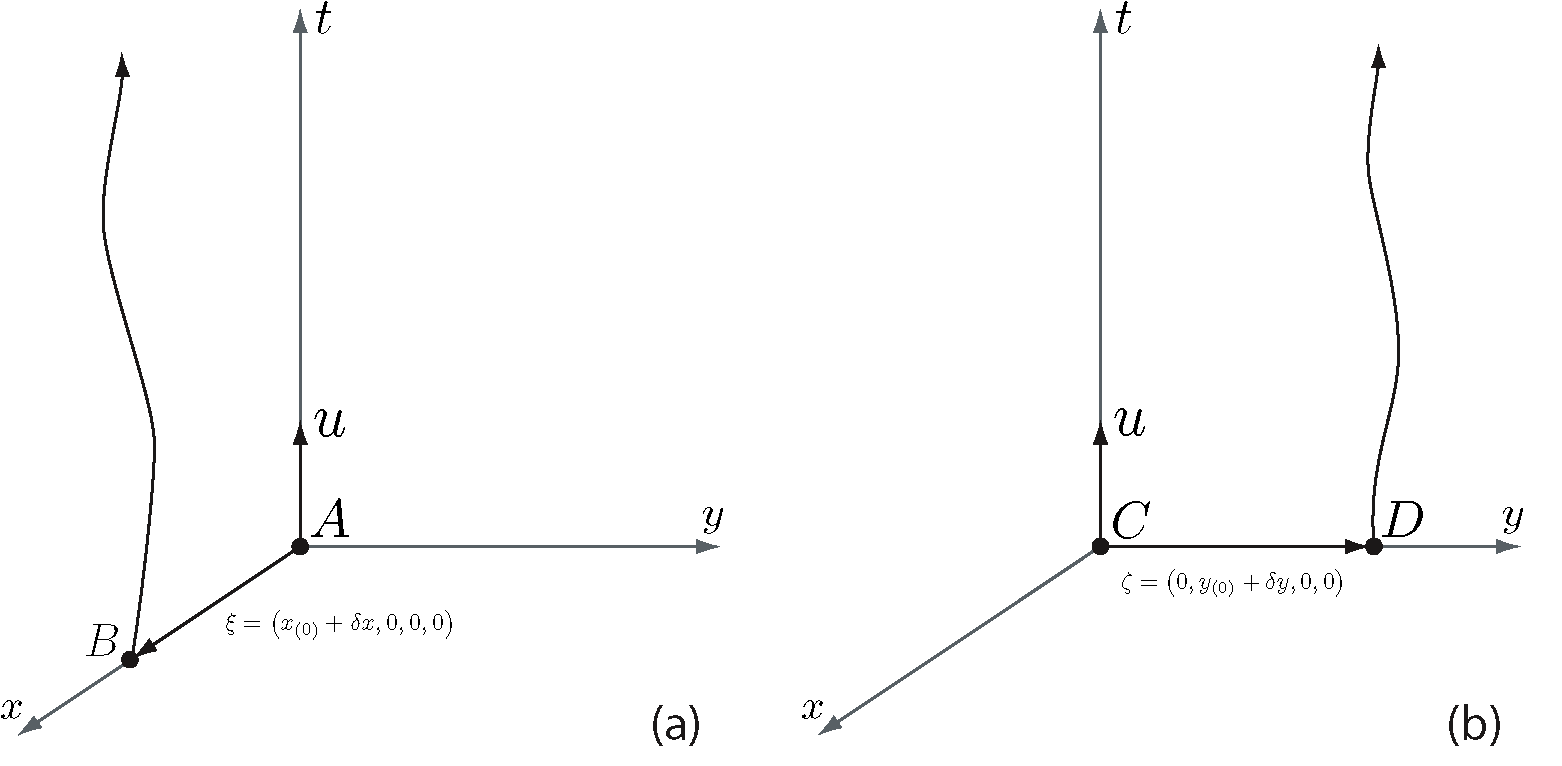
\includegraphics[width=\linewidth]{figures/inspiral/deviation}
\end{center}
\caption[Effect of a Gravitational Wave on Test Particles]{%
\label{f:particles}
The axes shown in (a) and (b) represent Local Lorentz frames for particles $A$
and $C$ respectively. The effect of a gravitational wave in these frame can be
described in terms of its effect on the vectors $\xi$ and $\zeta$ separating
the particles at the origin from particles $B$ and $D$.
}
\end{figure}

\begin{figure}[p]
\begin{center}
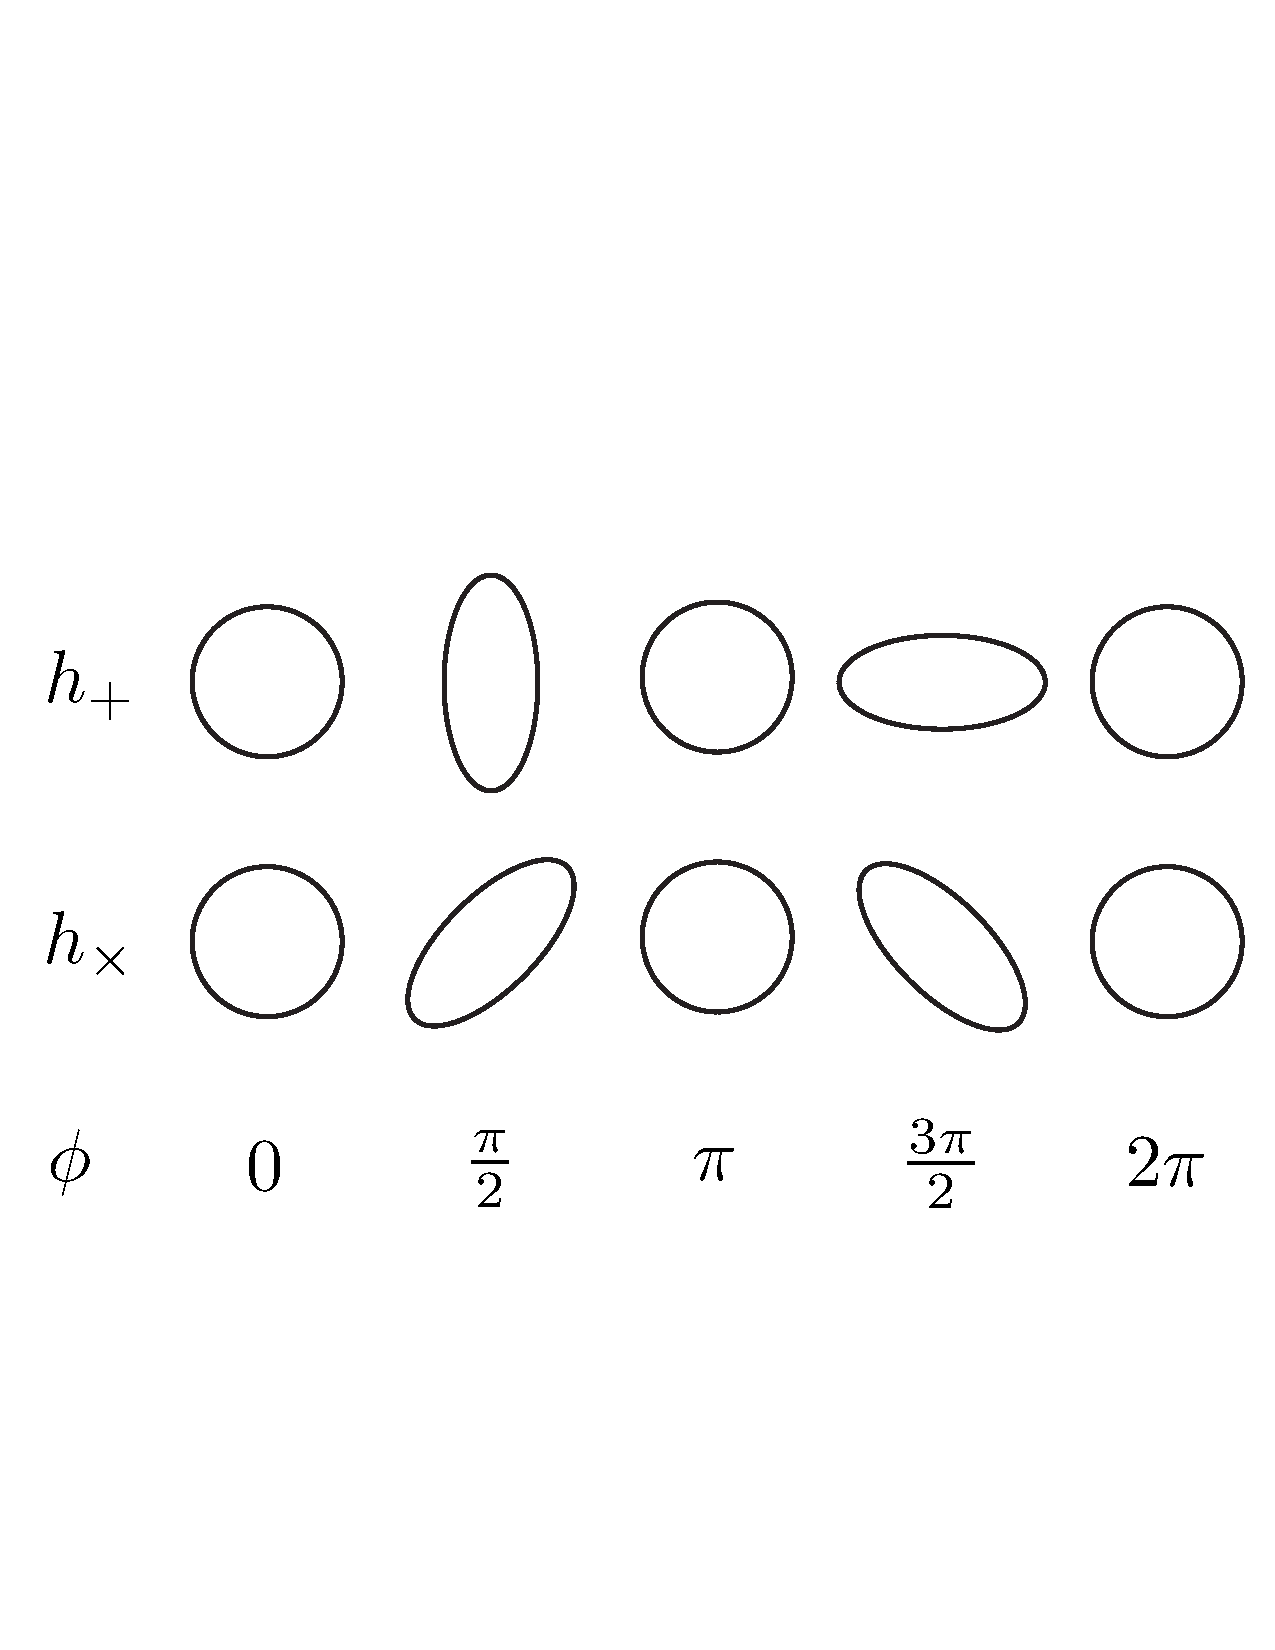
\includegraphics[width=\linewidth]{figures/inspiral/rings}
\end{center}
\caption[Effect of a Gravitational Wave Polarizations on a Ring of Particles]{%
\label{f:rings}
The effect of the two polarizations $h_+$ and $h_\times$ of a sinusoidal
gravitational wave propagating through the page on a ring of test particles.
As the phase $\phi$ of the gravitational wave changes through a complete
cycle, the rings are distorted.
}
\end{figure}

\begin{figure}[p]
\begin{center}
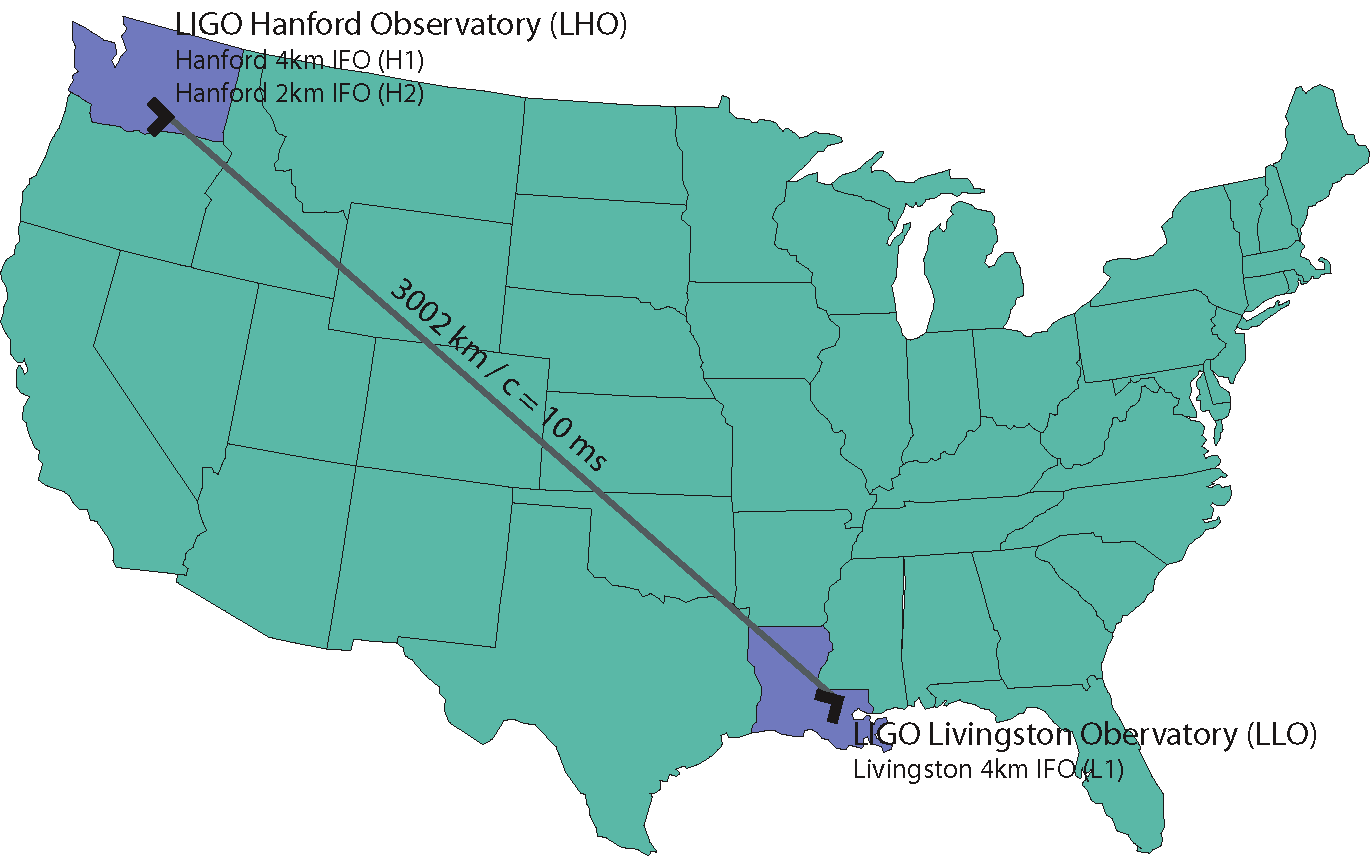
\includegraphics[width=\linewidth]{figures/inspiral/observatories}
\end{center}
\caption[Location of LIGO Interferometers]{%
\label{f:usmap}
The location of the three LIGO interferometers. There are two interferometers
at the LIGO Hanford Observatory (LHO) in Washington and one interferometer at
the LIGO Livingston Observatory in Louisiana.
}
\end{figure}

\begin{figure}[p]
\begin{center}
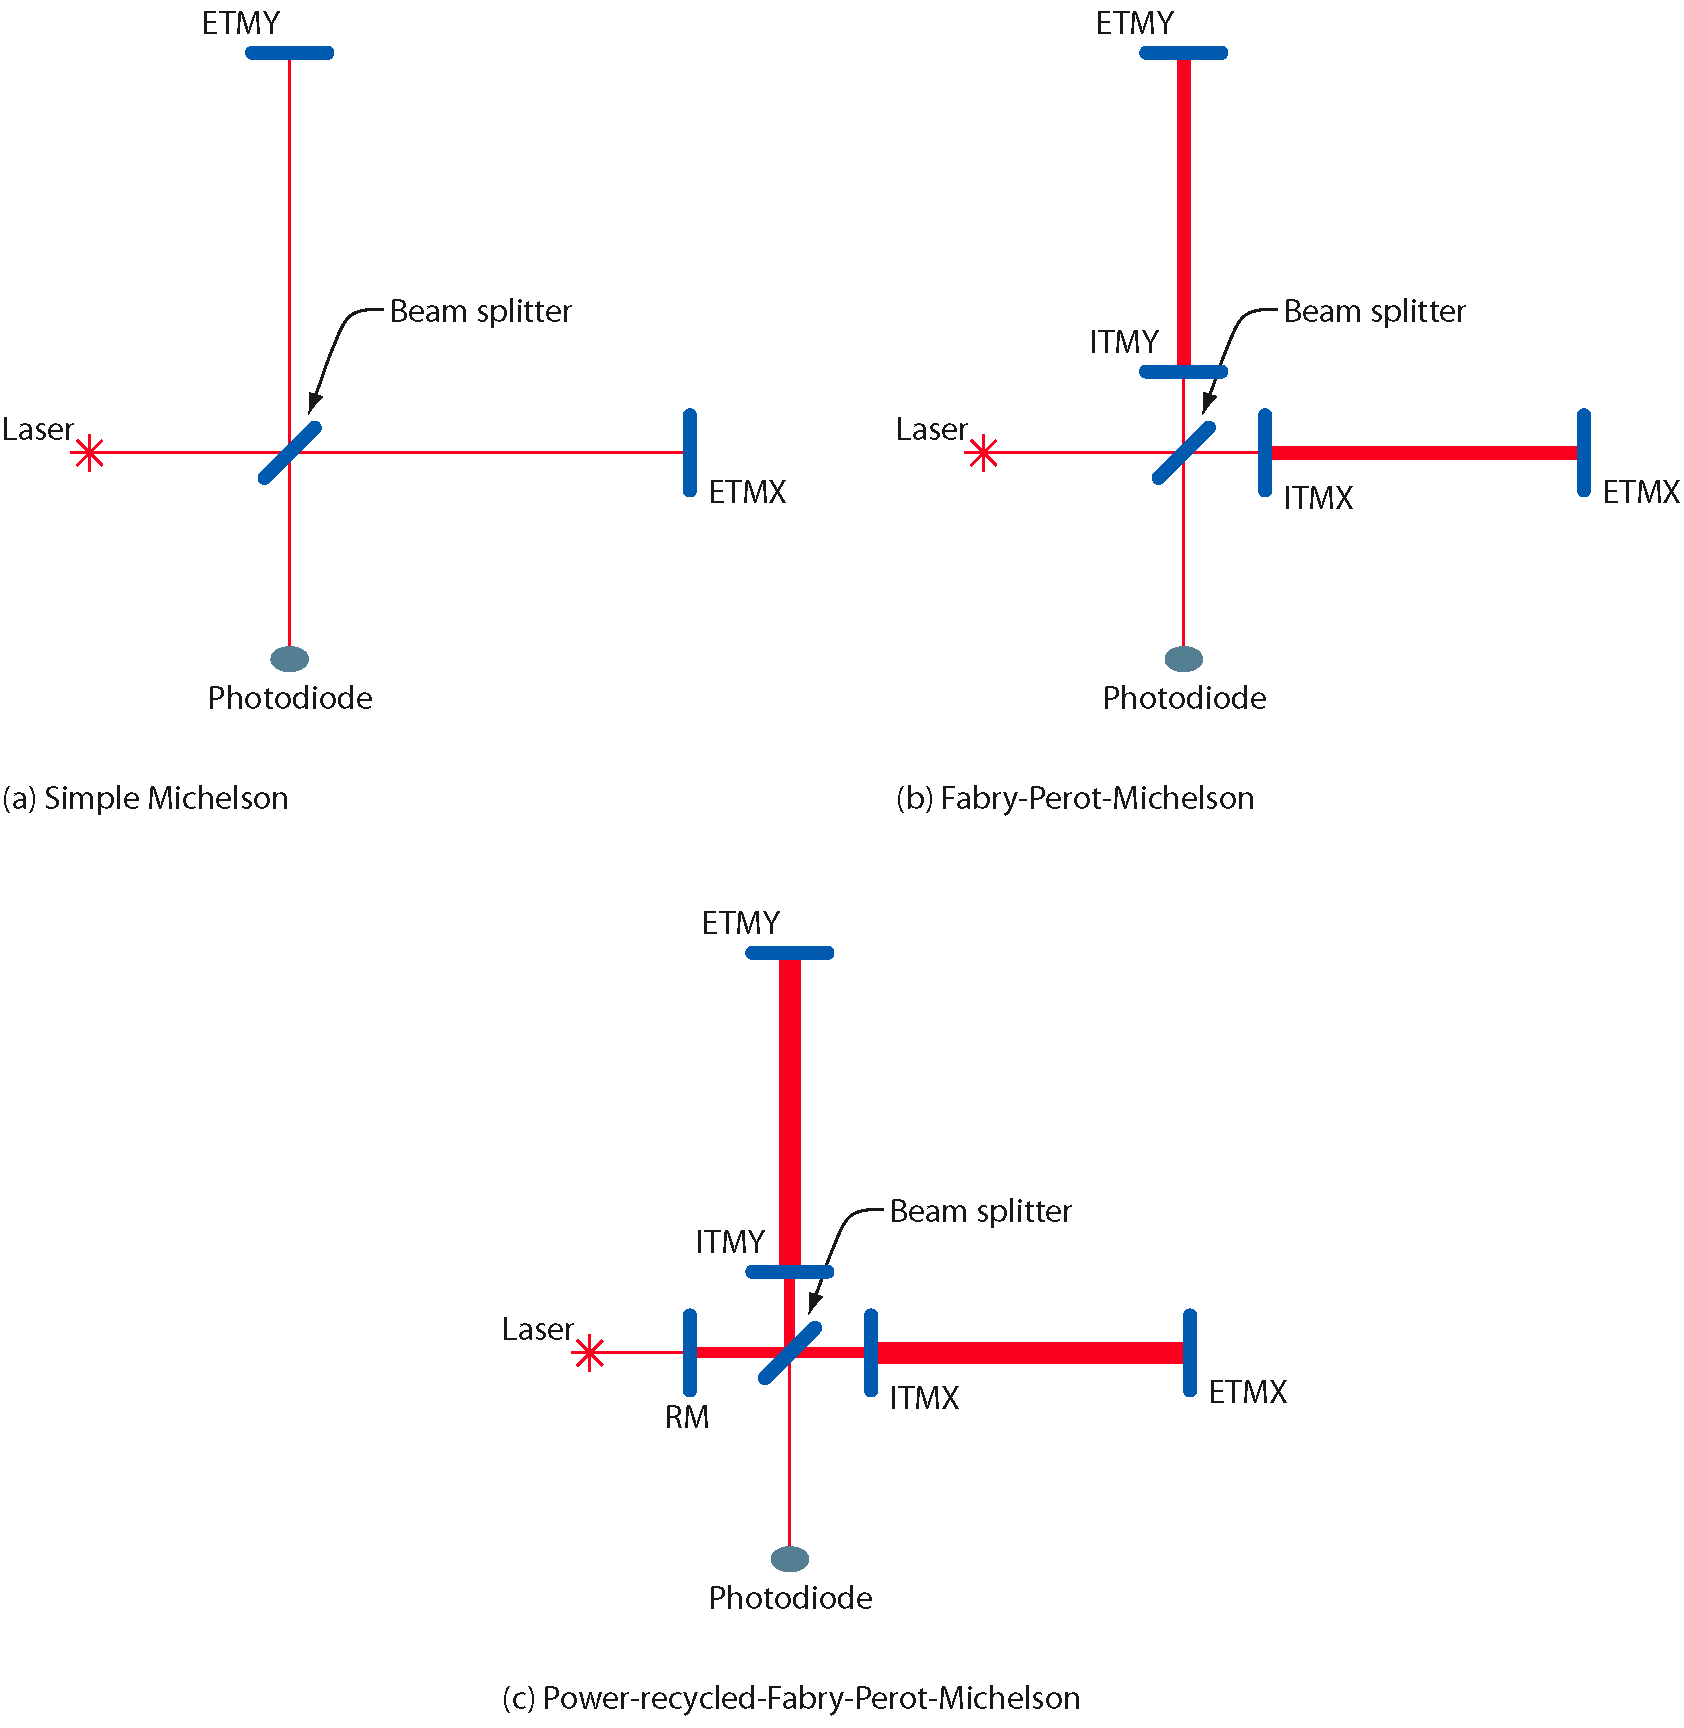
\includegraphics[width=\linewidth]{figures/inspiral/ifoconfigs}
\end{center}
\caption[Optical Configuration of LIGO]{%
\label{f:ifodesign}
The possible optical configurations of first generation laser interferometers.
The inner $x$ and $y$ test masses (mirrors) are denoted ITMX and ITMY
respectively, and the end $x$ and $y$ test masses (mirrors) are denoted ETMX
and ETMY respectively. The recycling mirror is denoted by RM.  Initial LIGO is
a power-recycled-Fabry-Perot interferometer, type (c) in this figure.
}
\end{figure}

\begin{figure}[p]
\begin{center}
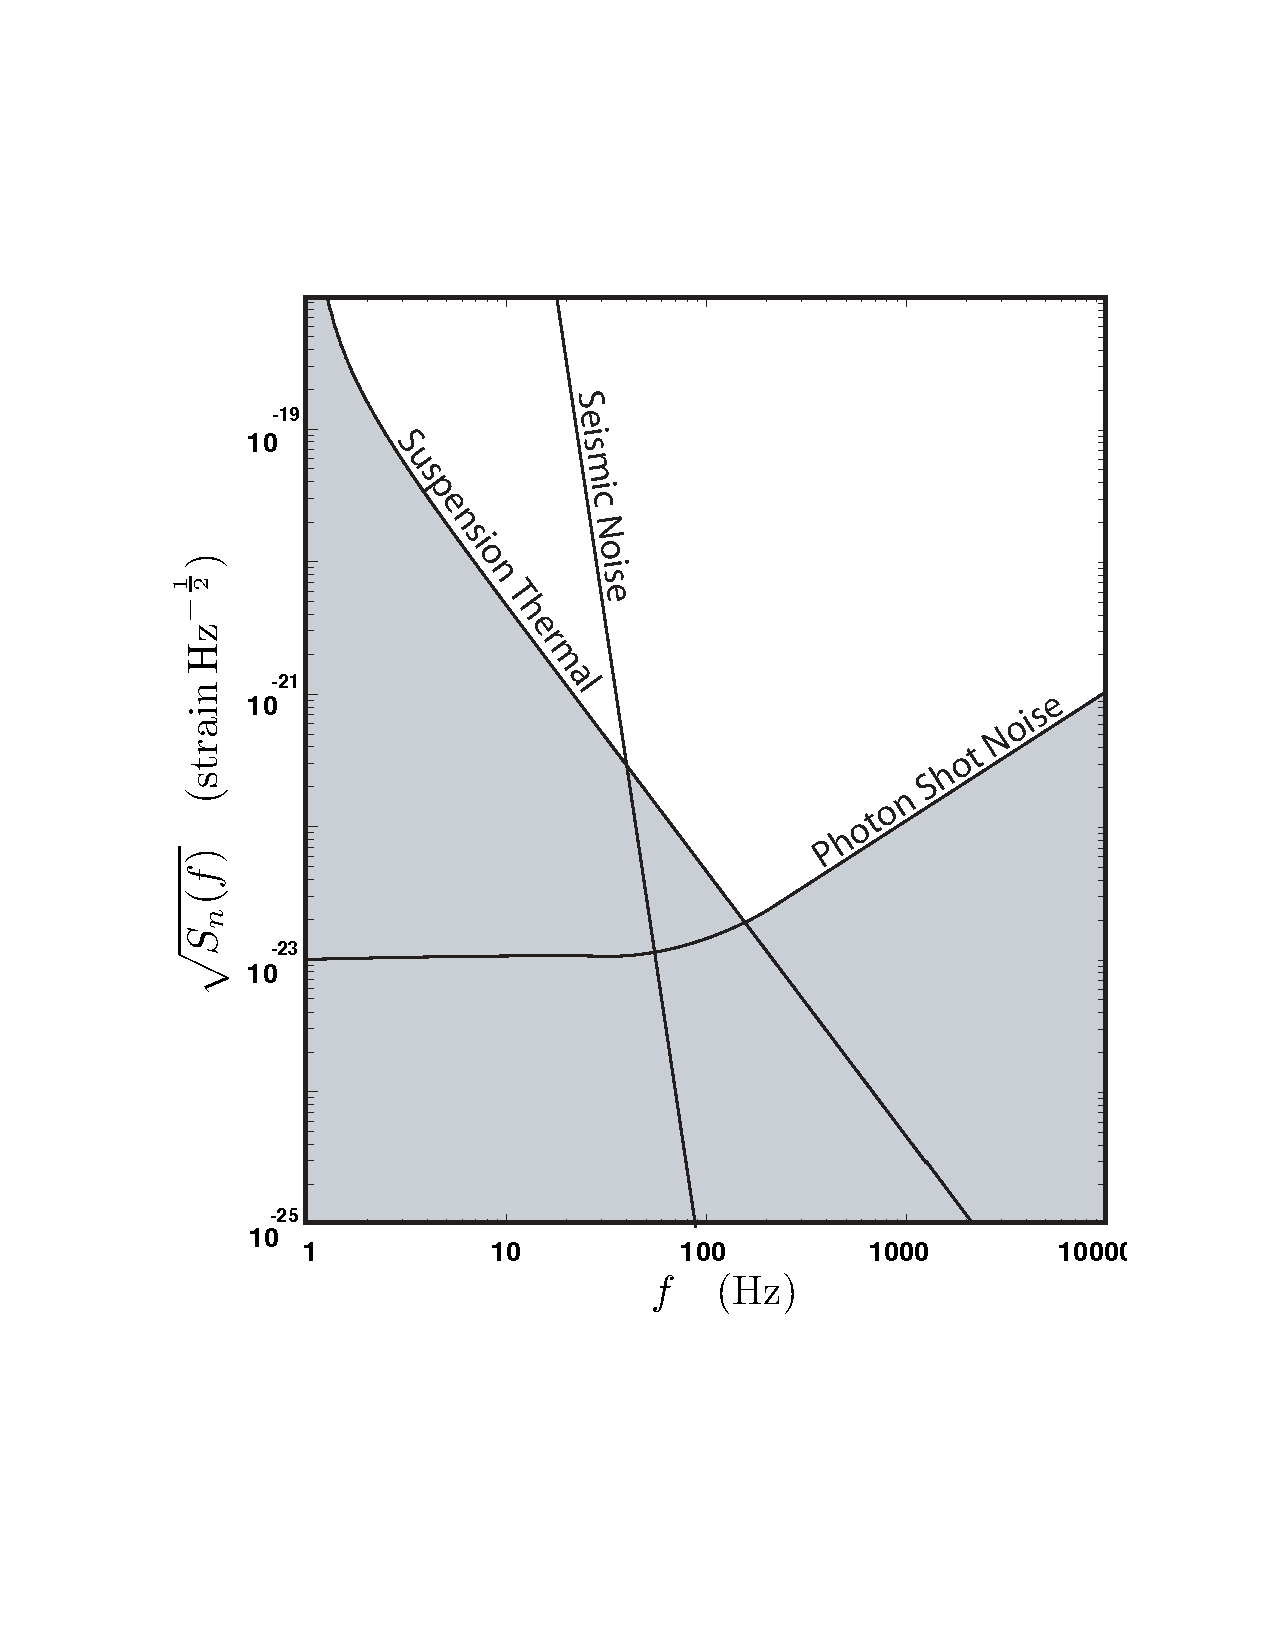
\includegraphics[width=\linewidth]{figures/inspiral/ligonoise}
\end{center}
\caption[Fundamental Noise Sources of Initial LIGO]{%
\label{f:design_noisecurve}
The fundamental noise sources of LIGO.
}
\end{figure}

\begin{figure}[p]
\begin{center}
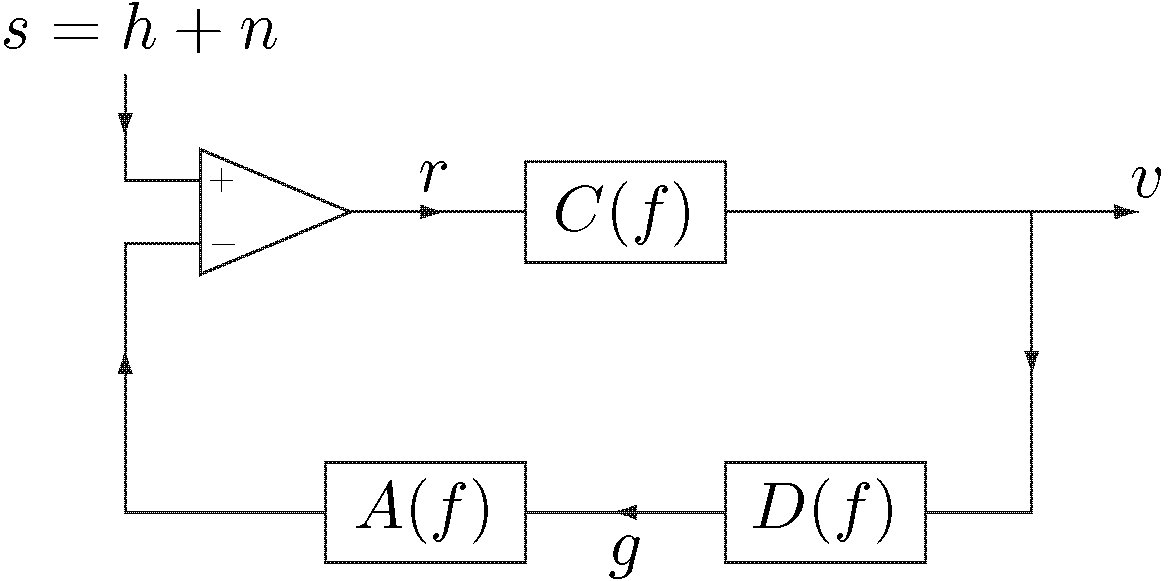
\includegraphics[width=\linewidth]{figures/inspiral/darm}
\end{center}
\caption[Differential mode control servo loop]{%
\label{f:darmloop}
The differential more servo control loop. The figure shows the positions of
three filters: the sensing function $C(f)$, the digital filter $D(f)$ and
the actuation function $A(f)$. The input signal is $s$ and the measured signal
is the error signal $v$. $r$ is the residual length of the cavity and $g$ is
the control signal.
}
\end{figure}

\begin{figure}[p]
\begin{center}
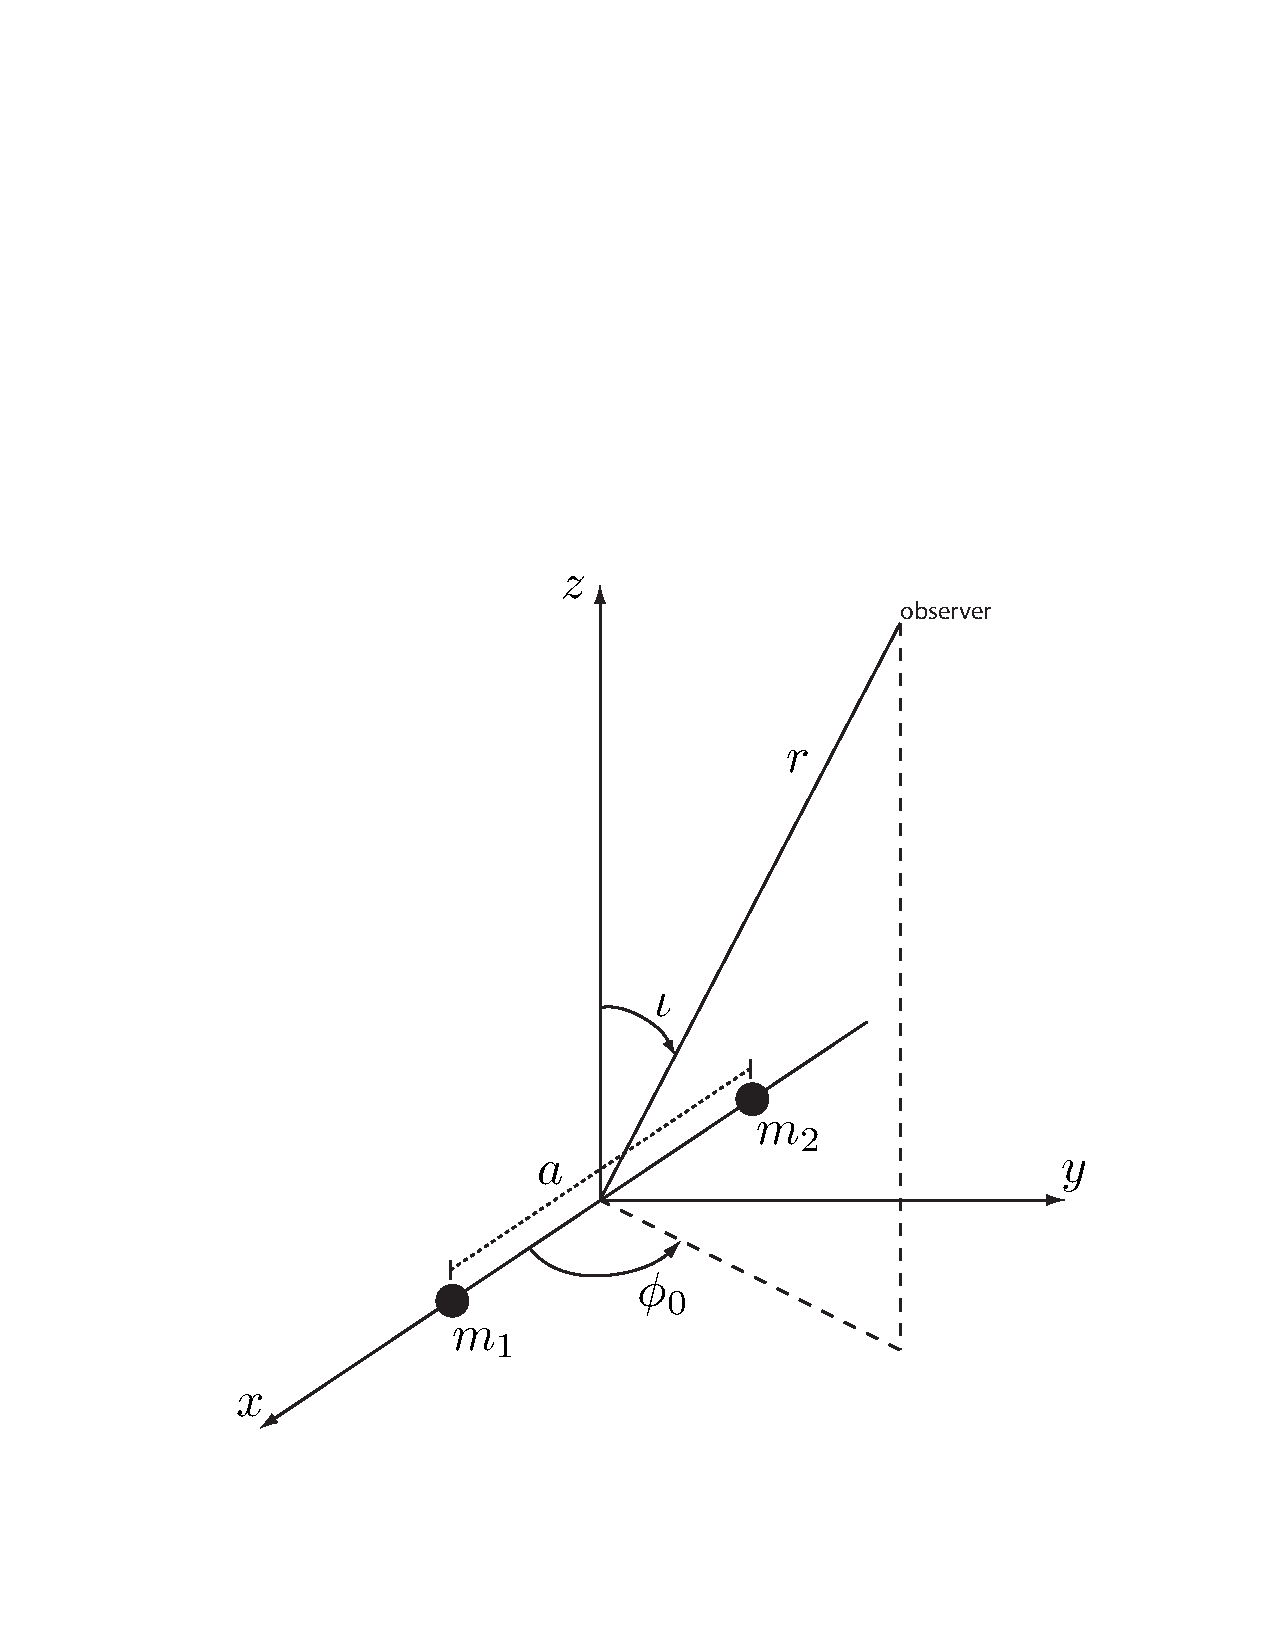
\includegraphics[width=\linewidth]{figures/inspiral/binary}
\end{center}
\caption[Coordinates Used to Describe Gravitational Radiation from a Binary]{%
\label{f:binary}
The parameters of a binary system with rotational axis aligned along the
$z$-axis.
}
\end{figure}

\begin{figure}[p]
\begin{center}
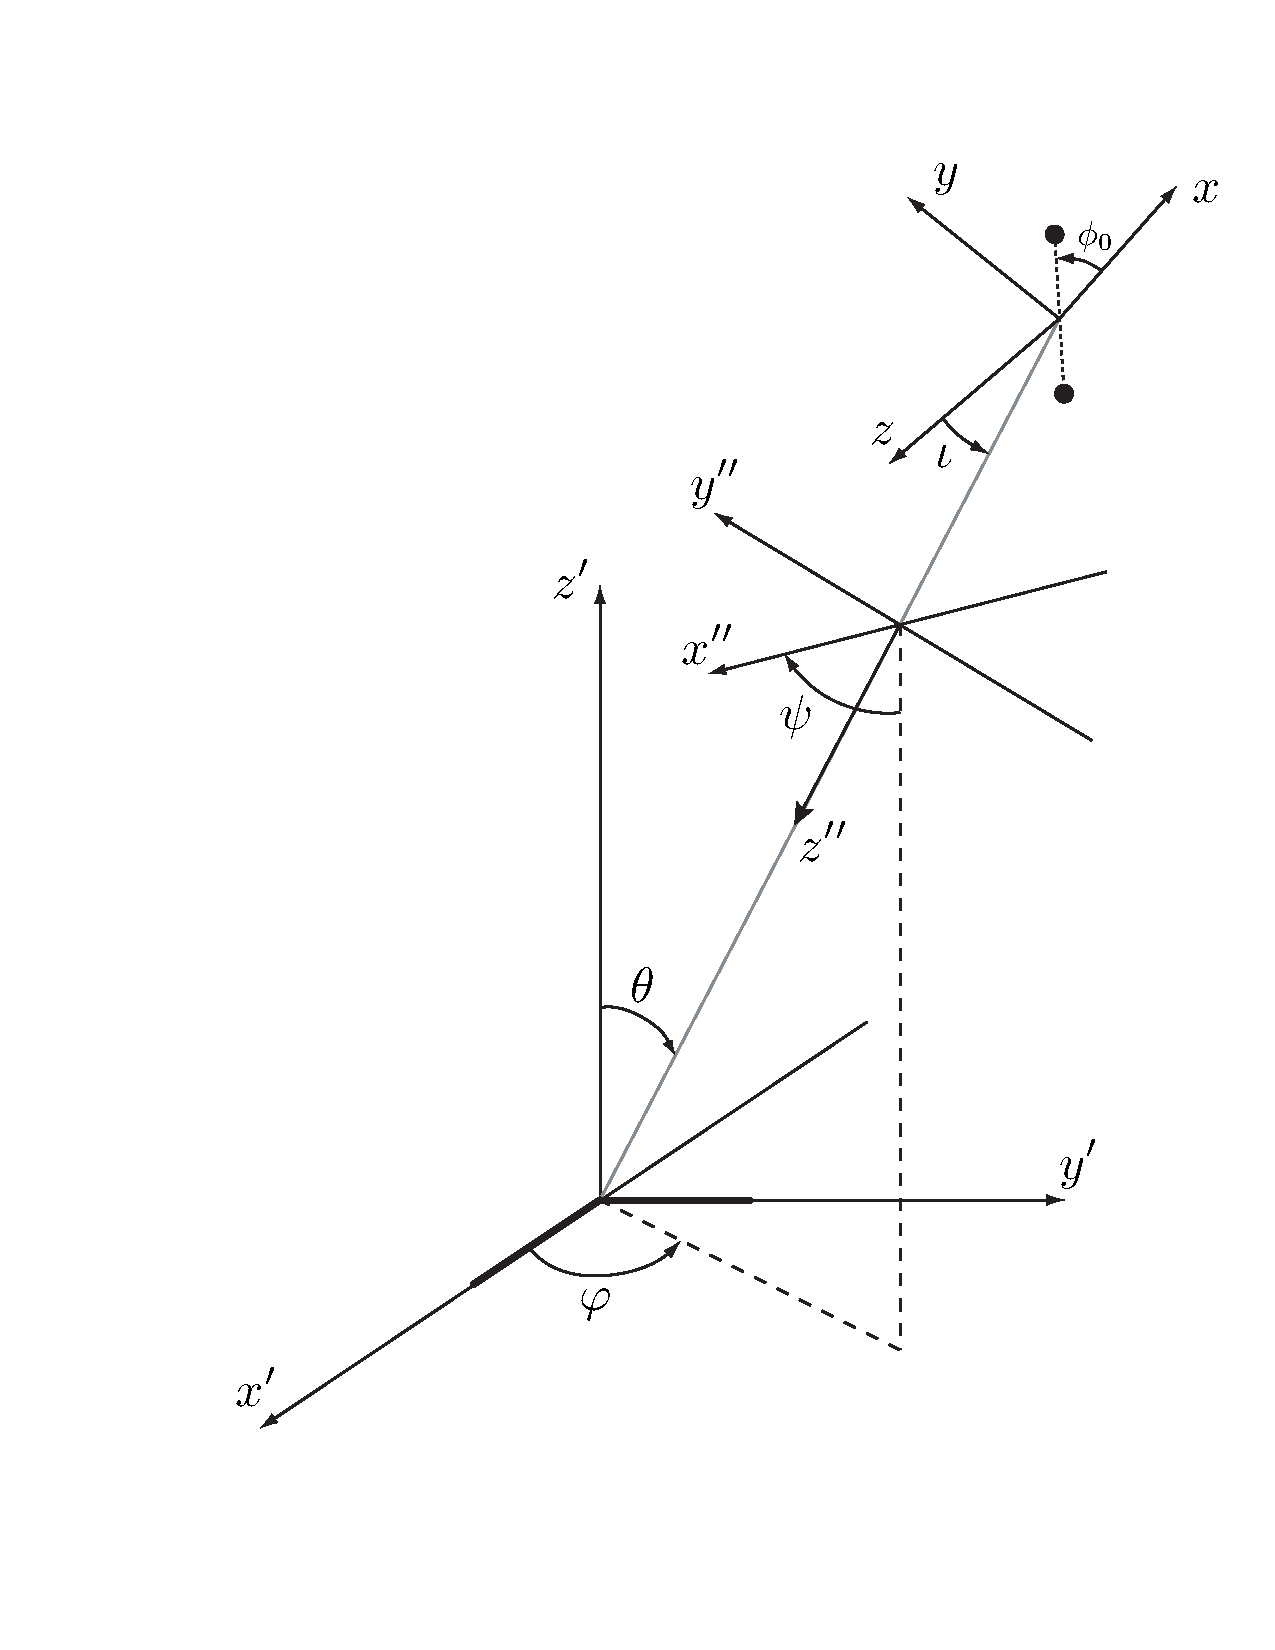
\includegraphics[width=\linewidth]{figures/inspiral/euler}
\end{center}
\caption[Coordinates Used to Describe the Response of a Gravitational Wave Interferometer]{%
\label{f:euler}
Euler angles of a binary system relative to the detector frame $x',y',z'$. The
frame of radiation basis is shown as $x''$ and $y''$.
}
\end{figure}

\begin{figure}[p]
\begin{center}
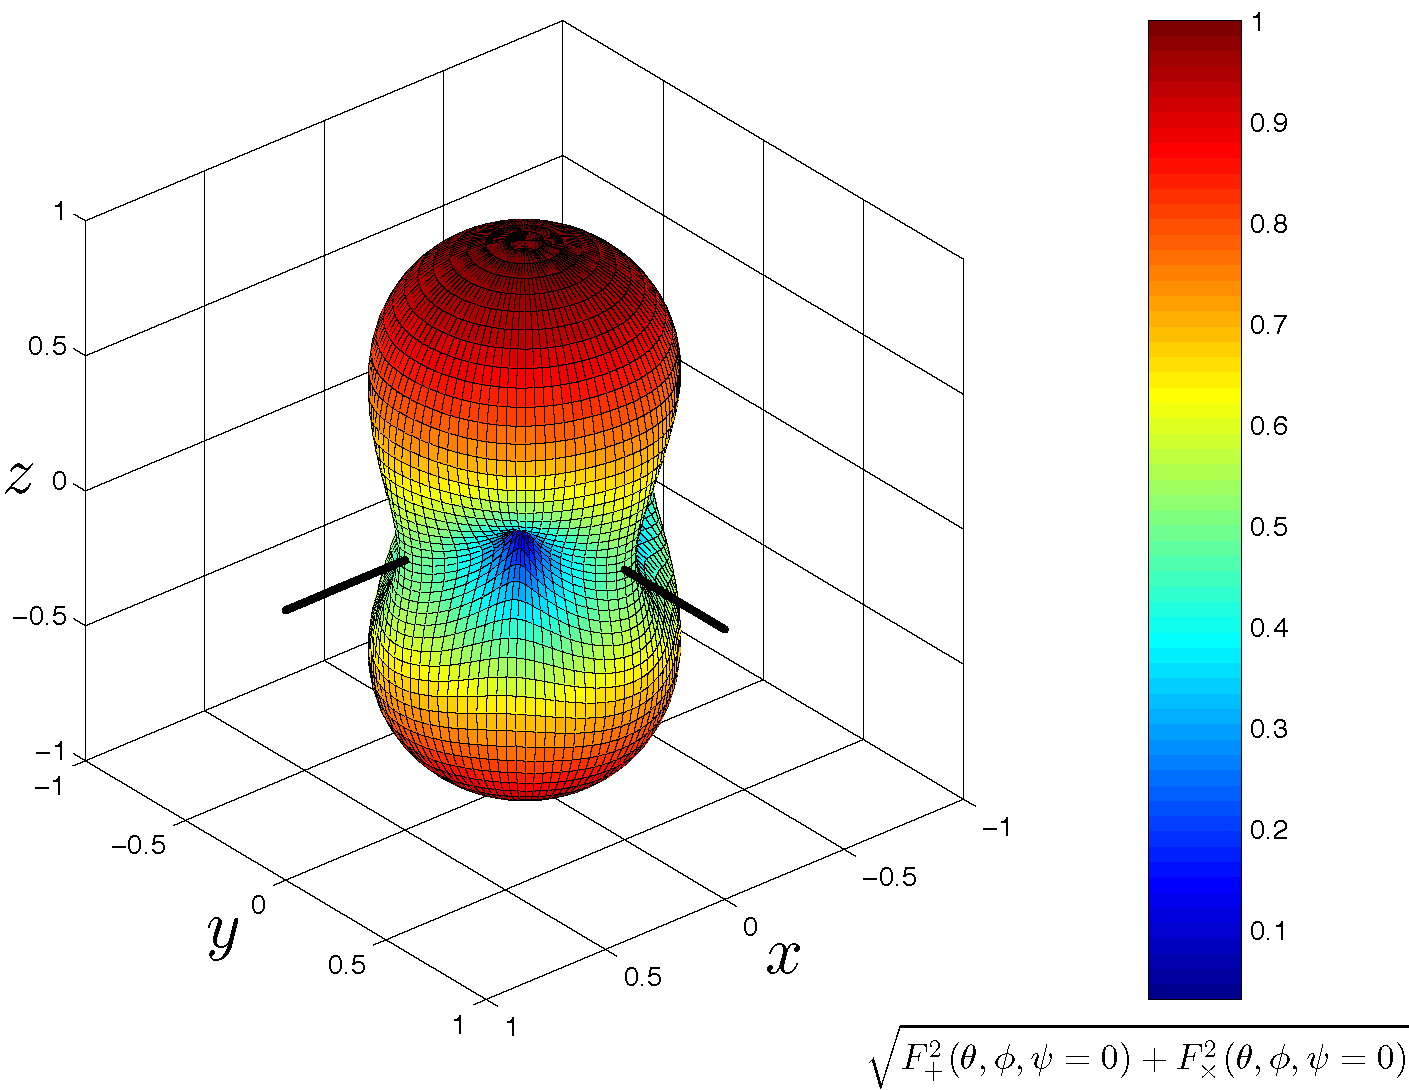
\includegraphics[width=\linewidth]{figures/inspiral/beampattern}
\end{center}
\caption[Antenna Response of an Interferometer]{%
\label{f:beampattern}
Level surface of the detector response function. The directions of the
interferometer arms are shown.
}
\end{figure}
